% ==============================================================================
% CivicShield AI ("מגן התודעה הלאומי") - Main LaTeX Entry Point
% Assignment 2: Preliminary Engineering & Academic Design Report
% University of Haifa | Applied AI & Vibe Coding (Dr. Yoram Segal)
% ==============================================================================
\documentclass{civicshield}

\begin{document}

% ==============================================================================
% TITLE PAGE (COVER)
% ==============================================================================
\begin{titlepage}
\thispagestyle{empty}
\begin{otherlanguage}{english}
\noindent
\begin{tikzpicture}[remember picture, overlay]
    % Deep Navy Full-Bleed Top Banner
    \fill[CivicNavy] (current page.north west) rectangle ([yshift=-11.8cm]current page.north east);
    % Gold & Teal Accent Bars
    \fill[CivicGold] ([yshift=-11.8cm]current page.north west) rectangle ([yshift=-12.02cm]current page.north east);
    \fill[CivicTeal] ([yshift=-12.02cm]current page.north west) rectangle ([yshift=-12.18cm]current page.north east);

    % Subtle geometric security grid in top banner
    \begin{scope}[shift={(current page.north west)}]
        \foreach \x in {0, 1.5, ..., 21} {
            \draw[CivicBlue, opacity=0.35, line width=0.4pt] (\x cm, 0) -- (\x cm, -11.8cm);
        }
        \foreach \y in {-1, -2.5, ..., -10} {
            \draw[CivicBlue, opacity=0.35, line width=0.4pt] (0, \y cm) -- (21cm, \y cm);
        }
    \end{scope}

    % Bottom Footer Strip
    \fill[CivicNavy] (current page.south west) rectangle ([yshift=2.2cm]current page.south east);
    \fill[CivicTeal] ([yshift=2.2cm]current page.south west) rectangle ([yshift=2.35cm]current page.south east);
    \node[text=white, text width=18cm, align=center, font=\sffamily\normalsize] at ([yshift=1.1cm]current page.south) {
        \textbf{\he{קורס:}} \he{יישומי בינה מלאכותית ו-\en{Vibe Coding} (שיעור 4: \en{Multi-Agent Orchestration})} \quad|\quad \textbf{\he{מרצה:}} \he{ד"ר יורם סגל}\\[4pt]
        \textbf{\he{מגיש הפרויקט:}} \en{ShmuelTetroashvili} \quad|\quad \textbf{\he{תאריך הפקה:}} \he{נובמבר 2026} \quad|\quad \textbf{\he{גרסה:}} \en{v1.0-RFP-FINAL}
    };
\end{tikzpicture}

\vspace*{-1.75cm}
\begin{center}
    % Top institutional tag in gold
    {\color{CivicGold}\sffamily\bfseries\large UNIVERSITY OF HAIFA \quad|\quad NATIONAL TENDER PRELIMINARY REPORT}\\[0.3cm]
    {\color{white}\sffamily\bfseries\large \he{אוניברסיטת חיפה — קורס יישומי \en{AI} ו-\en{Vibe Coding} (ד"ר יורם סגל)}}\\[0.55cm]

    % Vector CivicShield Emblem (pure TikZ)
    \begin{tikzpicture}[scale=0.88]
        % Outer Glow Circle
        \fill[CivicBlue!60!CivicNavy, opacity=0.45] (0,0) circle (2.25cm);
        \draw[CivicTeal, line width=1.4pt, dashed] (0,0) circle (2.05cm);
        % Main Shield Polygon
        \path[fill=CivicNavy!85!black, draw=CivicGold, line width=2pt]
            (0, 1.75) -- (1.45, 1.2) -- (1.35, -0.35) .. controls (1.1, -1.25) and (0.4, -1.65) .. (0, -1.85)
            .. controls (-0.4, -1.65) and (-1.1, -1.25) .. (-1.35, -0.35) -- (-1.45, 1.2) -- cycle;
        % Inner Teal Shield Accent
        \path[draw=CivicTeal, line width=1pt]
            (0, 1.48) -- (1.18, 1.0) -- (1.1, -0.3) .. controls (0.9, -1.02) and (0.32, -1.35) .. (0, -1.52)
            .. controls (-0.32, -1.35) and (-0.9, -1.02) .. (-1.1, -0.3) -- (-1.18, 1.0) -- cycle;
        % Multi-Agent Mesh Nodes inside Shield (5 Agents + Hub)
        \node[circle, fill=CivicGold, inner sep=2.8pt] (hub) at (0, 0.05) {};
        \node[circle, fill=CivicTeal, inner sep=2pt] (n1) at (0, 0.85) {};
        \node[circle, fill=CivicTeal, inner sep=2pt] (n2) at (0.75, 0.35) {};
        \node[circle, fill=CivicTeal, inner sep=2pt] (n3) at (0.5, -0.65) {};
        \node[circle, fill=CivicTeal, inner sep=2pt] (n4) at (-0.5, -0.65) {};
        \node[circle, fill=CivicTeal, inner sep=2pt] (n5) at (-0.75, 0.35) {};
        \draw[CivicTeal!80!white, line width=0.8pt] (hub)--(n1) (hub)--(n2) (hub)--(n3) (hub)--(n4) (hub)--(n5);
        \draw[CivicGold!70!white, line width=0.6pt, opacity=0.75] (n1)--(n2)--(n3)--(n4)--(n5)--(n1);
    \end{tikzpicture}

    \vspace{0.25cm}
    {\color{white}\sffamily\bfseries\Huge CivicShield AI}\\[0.25cm]
    {\color{CivicGold}\sffamily\bfseries\LARGE \he{מגן התודעה הלאומי}}
\end{center}

\vspace{2.25cm}
\begin{center}
    {\color{CivicNavy}\sffamily\bfseries\Large \he{דוח מכין (\en{Preliminary Design Report}) להקמת מערכת רב-סוכנית לאומית}}\\[0.25cm]
    {\color{CivicBlue}\sffamily\bfseries\large \he{להגנה על הספרה הציבורית, זיהוי מניפולציות תודעה ושמירה על טוהר הבחירות}}\\[0.45cm]
    {\color{CivicSlate}\sffamily\normalsize \he{סינתזה בין-תחומית: מדעי המדינה, תקשורת פוליטית והנדסת מערכות \en{Multi-Agent AI}}}
\end{center}

\vspace{0.55cm}
\begin{center}
\begin{tcolorbox}[colback=CivicGrayBg, colframe=CivicNavy, width=0.92\textwidth, arc=4pt, boxrule=1pt, left=12pt, right=12pt, top=10pt, bottom=10pt]
\begin{otherlanguage}{hebrew}
\textbf{\textcolor{CivicNavy}{מענה למכרז ממשלתי משותף (מדומיין לצורכי המטלה):}}
ועדת הבחירות המרכזית (CEC), מערך הסייבר הלאומי (INCD) ומשרד המשפטים.\\[4pt]
\textbf{\textcolor{CivicNavy}{פרדיגמת התכנון:}}
חיסון תודעתי פרואקטיבי (\en{Cognitive Prebunking}), ניתוח מסגור פוליטי, זיהוי רשתות בוטים ו-\en{Deepfakes} באמצעות ועדת סוכני \en{AI} מתואמת, תחת הפרדת רשויות ופיקוח שיפוטי משולש (\en{Human-in-the-Loop}).\\[4pt]
\textbf{\textcolor{CivicNavy}{מתודולוגיית הכנה:}}
ועדת מומחים של 5 סוכנים אוטונומיים (\en{Master, Theory, Architect, Simulator, RedTeam}) לפי עקרונות שיעור 4, בשילוב סימולציות כמותיות ב-\en{Python} וגרפיקה וקטורית ב-\en{TikZ}.
\end{otherlanguage}
\end{tcolorbox}
\end{center}

\end{otherlanguage}
\end{titlepage}

% ==============================================================================
% PAGE 2: DOCUMENT CONTROL & TENDER METADATA
% ==============================================================================
\clearpage
\chapter*{בקרת מסמך, מפרט המכרז ותקציר מנהלים מוסדי}
\addcontentsline{toc}{chapter}{בקרת מסמך, מפרט המכרז ותקציר מנהלים מוסדי}

\begin{rfpbox}[זהות ההגשה ונתוני ייחוס מכרזיים]
מסמך זה מהווה את \textbf{הדוח המכין (Preliminary Engineering \& Academic Design Report)} במסגרת מטלה 2 בקורס יישומי \en{AI} באוניברסיטת חיפה. המסמך בנוי במתכונת של תיק מכרז ממשלתי מחייב, המפרט את ההיתכנות התיאורטית, האדריכלות ההנדסית, המודלים המתמטיים, המגבלות החוקתיות והתקציב להקמת מערכת \en{CivicShield AI} ("מגן התודעה הלאומי").
\end{rfpbox}

\vspace{0.2cm}
{\renewcommand{\arraystretch}{1.35}
\begin{tabularx}{\textwidth}{|p{4.3cm}|X|}
\hline
\textbf{\textcolor{CivicNavy}{שדה בקרה}} & \textbf{\textcolor{CivicNavy}{פירוט מחייב}} \\ \hline
שם הפרויקט והמערכת & \en{CivicShield AI} — מערכת לאומית להגנת הספרה הציבורית וטוהר הבחירות \\ \hline
מזהה תיק ומהדורה & \en{GOV-IL-RFP-2026-CSAI} \quad|\quad מהדורה \en{1.0} (דוח מכין סופי) \\ \hline
גופים מזמינים (משולב) & ועדת הבחירות המרכזית, מערך הסייבר הלאומי, הייעוץ המשפטי לממשלה \\ \hline
דיסציפלינות ליבה & תקשורת פוליטית, מדעי המדינה, הנדסת \en{Multi-Agent AI}, סייבר ומשפט חוקתי \\ \hline
סוג המסמך ואופיו & מסמך אפיון והיתכנות קודם-מימוש (\en{Pre-Implementation Specification}) \\ \hline
ארכיטקטורת תיעוד & מודולרית ב-\en{LuaLaTeX} (\en{civicshield.cls}), 8 פרקים, 6 גרפי \en{Python}, תרשימי \en{TikZ} \\ \hline
סטטוס אישור ועדת סוכנים & אושר לאחר ביקורת צוות אדום (\en{Red Team Audit Pass \#2}) — ללא ממצאים קריטיים \\ \hline
\end{tabularx}}

\vspace{0.5cm}
\section*{תקציר אקדמי והנדסי (Abstract)}
המעבר המואץ של השיח הפוליטי אל פלטפורמות אלגוריתמיות ריכוזיות, לצד הזמינות הגוברת של מודלי שפה גדולים (\en{LLMs}) וכלי סינתזה אודיו-ויזואליים (\en{Deepfakes}), שינה באופן מבני את פגיעותן של דמוקרטיות מודרניות. מבצעי השפעה זרים (\en{Foreign Information Manipulation and Interference -- FIMI}) ורשתות בוטים אוטונומיות מסוגלים כיום לעצב את סדר היום התקשורתי, להקצין מסגרות פרשנות ולהפעיל "עוצמה חדה" (\en{Sharp Power}) בקצבים החורגים מיכולת התגובה של בדיקת עובדות אנושית בדיעבד (\en{Reactive Fact-Checking}).

דוח מכין זה מציג תכנון שלם למערכת \en{CivicShield AI}, המבוססת על פרדיגמה כפולה: \textbf{(1) חיסון תודעתי פרואקטיבי (\en{Cognitive Prebunking})} המעביר תגובה מהרשאה מאוחרת אל הקדמת התודעה טרם חשיפה לנרטיב כוזב; ו-\textbf{(2) תזמור רב-סוכני מתואם (\en{Multi-Agent Committee})} המפריד בין סוכני ניטור, סוכני מסגור תקשורתי, סוכני אימות פורנזי וסוכן בקרה חוקתי. במישור התיאורטי, המערכת ממפה תיאוריות קלאסיות בתקשורת ובמדעי המדינה — ובהן \en{Agenda Setting}, \en{Framing}, \en{Spiral of Silence}, המרחב הציבורי של \en{Habermas} ו"דמוקרטיה מתגוננת" — לכדי צינורות חישוב מוגדרים היטב. במישור הכמותי, הדוח גוזר ומריץ ארבעה מודלים מתמטיים מרכזיים ב-\en{Python}: מודל הדבקה תודעתית (\en{SIRI ODEs}), דינמיקת קיטוב תחומת-אמון (\en{Hegselmann-Krause}), איחוד פורנזי בייסיאני לזיהוי \en{Deepfake}, ומודל תורים \en{M/M/c} לחיזוי זמני תגובה ביום הבחירות. לבסוף, המסמך מעגן הגנות חוקתיות קשיחות, ובראשן מנגנון חתימה קריפטוגרפית משולש המבטיח כי בינה מלאכותית תוכל \emph{לזהות ולהמליץ}, אך לעולם לא לצנזר אזרחים באופן אוטונומי.

% ==============================================================================
% FRONT MATTER LISTS (TOC, LOF, LOT)
% ==============================================================================
\clearpage
\tableofcontents

\clearpage
\listoffigures
\vspace{0.8cm}
\listoftables

% ==============================================================================
% CORE REPORT CHAPTERS (8 MODULAR CHAPTERS)
% ==============================================================================
% ==============================================================================
% Chapter 1: Executive Summary, Tender Context & Operational Concept (CONOPS)
% ==============================================================================
\chapter{תקציר מנהלים, רקע המכרז וחוזה ההקמה הלאומי}
\label{ch:executive}

\section{פתח דבר: הדמוקרטיה הדליברטיבית בעידן הלוחמה התודעתית}
מערכות בחירות דמוקרטיות ומוסדות שלטון נציגיים נשענים מאז ומעולם על תשתית אפיסטמית משותפת: יכולתם של אזרחים לקבל מידע אמין, לנהל דיון ציבורי חופשי בספרה הציבורית (\en{Public Sphere}), ולגבש הכרעה מושכלת בקלפי. ואולם, בעשור האחרון חל שינוי מבני עמוק באופי הזירה הציבורית. השילוב בין אלגוריתמים של רשתות חברתיות המתגמלים זעם וקיטוב (\en{Engagement-Driven Amplification}), לבין זמינותם של מודלי שפה גדולים (\en{LLMs}) וכלי סינתזה מולטי-מודאליים (\en{Deepfakes}), העניק לגורמים עוינים — מדינתיים ושאינם מדינתיים — יכולת חסרת תקדים להנדס את השיח הלאומי בזמן אמת \cite{vosoughi2018, walker2018}.

מבצעי השפעה זרים (\en{Foreign Information Manipulation and Interference -- FIMI}) אינם מסתפקים עוד בהפצת ידיעה כוזבת נקודתית. במקום זאת, מערכי השפעה מודרניים מפעילים "נחילי תודעה": אלפי חשבונות מזויפים המופעלים בתיאום סינכרוני, מניעים הסטה מלאכותית של סדר היום (\en{Agenda Hijacking}), מזריקים מסגרות פרשנות מקטבות (\en{Polarizing Frames}), ומפיצים הקלטות קוליות או סרטוני וידאו מזויפים בשעות הקריטיות שטרם סגירת הקלפיות. במצב זה, מנגנוני התגובה המסורתיים של \textbf{בדיקת עובדות בדיעבד (\en{Reactive Fact-Checking})} נכשלים מבחינה מתמטית ותקשורתית: בעוד צוות עיתונאי נדרש שעות לאמת ולהפריך טענה, הנרטיב הכוזב מתפשט במהירות הגדולה פי שישה ממידע מאומת \cite{vosoughi2018}, ומותיר משקע תודעתי מתמשך (\en{Continued Influence Effect}).

\begin{rfpbox}[ייעוד המסמך והצהרת כשירות למכרז הלאומי]
דוח מכין זה מוגש כמענה רשמי למכרז הבין-משרדי \en{GOV-IL-RFP-2026-CSAI} מטעם \textbf{ועדת הבחירות המרכזית}, \textbf{מערך הסייבר הלאומי} ו\textbf{משרד המשפטים}. מטרת המסמך להוכיח היתכנות אקדמית, הנדסית, כמותית וחוקתית להקמת מערכת \en{CivicShield AI} ("מגן התודעה הלאומי") — תשתית לאומית לחיסון תודעתי פרואקטיבי (\en{Cognitive Prebunking}) המבוססת על ועדת סוכני \en{AI} מתואמת, תחת פיקוח שיפוטי משולש השולל כל אפשרות לצנזורה אוטומטית.
\end{rfpbox}

\section{ניתוח הפער האסטרטגי: מבדיקת עובדות בדיעבד לחיסון פרואקטיבי}
הפרדיגמה הרווחת כיום בגופי רגולציה ובמערכות חדשות מבוססת על מעגל תגובה לינארי ואיטי: (א) ידיעה כוזבת עולה לרשת; (ב) היא צוברת חשיפה ויראלית במשך שעות; (ג) הציבור מתבצר בעמדות רגשיות; ו-(ד) רק לאחר שהנזק התרחש מתפרסמת הפרכה פוסט-פקטום. מחקרים עדכניים בפסיכולוגיה פוליטית מלמדים כי הפרכה מאוחרת אף עלולה לחזק את האמונה השקרית בקרב קהלים מקוטבים (\en{Backfire / Familiarity Effect}).

מערכת \en{CivicShield AI} מחליפה פרדיגמה זו בתיאוריית \textbf{החיסון התודעתי (\en{Psychological Inoculation / Prebunking})} \cite{mcguire1961, roozenbeek2022}. כשם שחיסון ביולוגי חושף את מערכת החיסון לגרסה מוחלשת של נגיף כדי לייצר נוגדנים בטרם ההדבקה, כך \en{CivicShield AI} מאתרת דפוסי מניפולציה בעודם באיבם (שלב ה-\en{Weak Signals} בקהילות סגורות וטלגרם), ומסייעת לגורמי ציבור מוסמכים לשדר לאזרחים "נוגדנים קוגניטיביים" — הסבר קצר, ניטרלי ובלתי מפלגתי החושף את \emph{הטכניקה הרטורית} של המניפולציה טרם הגעתה לזרם המרכזי.

{\renewcommand{\arraystretch}{1.35}
\begin{table}[htbp]
\centering
\caption{השוואה אסטרטגית בין הגישה המסורתית לגישת CivicShield AI}
\label{tab:paradigm_shift}
\begin{tabularx}{\textwidth}{|p{3.4cm}|X|X|}
\hline
\textbf{\textcolor{CivicNavy}{ממד השוואה}} & \textbf{\textcolor{CivicNavy}{גישה מסורתית (בדיקת עובדות בדיעבד)}} & \textbf{\textcolor{CivicNavy}{גישת CivicShield AI (חיסון פרואקטיבי)}} \\ \hline
תזמון התערבות & לאחר ויראליות שיא (תגובה מאוחרת בשעות או ימים) & בזמן התהוות דפוס ההשפעה (התראה תוך שניות וחיסון מוקדם) \\ \hline
מוקד הניתוח & אימות עובדתי נקודתי של משפט בודד & זיהוי קמפיין מתואם (\en{CIB}), מסגור מפלג וטופולוגיית בוטים \\ \hline
מנגנון הגנה קוגניטיבי & תיקון שגיאה לאחר היווצרות הטיה רגשית & הקניית עמידות לטכניקת ההונאה (\en{Prebunking}) \cite{roozenbeek2022} \\ \hline
מדרגיות הנדסית & תלויה בצוואר בקבוק של עורכים אנושיים & ועדת סוכני \en{AI} היררכית (\en{Multi-Agent Mesh}) + בקרה אנושית \\ \hline
מגבלה חוקתית & סיכון לשרירותיות רגולטורית בהסרת תוכן & איסור אכיפה ללא חתימה משולשת; הפרדה בין זיהוי לסמכות שיפוט \\ \hline
\end{tabularx}
\end{table}}

\section{תפיסת ההפעלה המבצעית (CONOPS)}
תפיסת ההפעלה הלאומית (\en{Concept of Operations -- CONOPS}) של מערכת \en{CivicShield AI} מתארת מחזור חיים סגור בן ארבעה שלבים רציפים הפועל 24/7 ומתגבר לקצב תגובה תחת \en{250ms} בתקופת 90 הימים שלפני בחירות ארציות:
\begin{enumerate}
    \item \textbf{איסוף ונירמול פומבי מאומת (\en{Privacy-Preserving Public Ingestion}):} המערכת צורכת אך ורק מידע פומבי גלוי (\en{OSINT}) מערוצי טלגרם ציבוריים, פוסטים ציבוריים ברשתות חברתיות ופידים חדשותיים. אין כל גישה להודעות פרטיות, שיחות אישיות או מידע מזהה של אזרחים מן השורה, והנתונים עוברים מיסוך אנונימי תחת תקן פרטיות דיפרנציאלית (\en{$\epsilon$-Differential Privacy}).
    \item \textbf{תזמור ניתוח רב-סוכני (\en{Multi-Agent Diagnostic Reasoning}):} הנתונים מוזרמים למרכז תזמור סוכנים (\en{Agent Mesh Hub}), שבו פועלים במקביל סוכן רשת ובוטים (\en{Network Agent}), סוכן מסגור תקשורתי (\en{Framing Agent}), סוכן אימות פורנזי (\en{Deepfake Multimodal Agent}) וסוכן תחזית אפידמיולוגית (\en{SIRI Simulation Agent}).
    \item \textbf{שיפוט חוקתי ושער אדם (\en{Constitutional Gate \& Triple-Signature}):} כל ממצא המדורג ברמת חומרה גבוהה מועבר ל\textbf{סוכן הבקרה החוקתי} הבודק התאמה לעקרונות חופש הביטוי, ההסתברות לשיוך זר (\en{FIMI Attribution}) והסכנה לטוהר הבחירות. הפעלת המלצת חסימה או תיוג דורשת חתימה דיגיטלית משולשת של גורמים מוסמכים.
    \item \textbf{תגובה מאוזנת: התראה והנגשת חיסון תודעתי:} המערכת אינה מוחקת דעות פוליטיות לגיטימיות. היא מנפיקה לכלי התקשורת, לוועדת הבחירות ולציבור דוחות שקיפות טכניים ומסרי \en{Prebunking} אובייקטיביים החושפים טכניקות מניפולציה מזוהות.
\end{enumerate}

איור~\ref{fig:conops_ch1} מציג את תפיסת ההפעלה מקצה לקצה במבנה זרימה וקטורי.

\begin{figure}[htbp]
\begin{tikzhebrew}
\begin{tikzpicture}[
    node distance=0.85cm and 0.65cm,
    stage/.style={rectangle, rounded corners=4pt, draw=CivicNavy, fill=CivicGrayBg, line width=1pt, minimum width=3.1cm, minimum height=1.65cm, align=center, font=\small},
    hub/.style={rectangle, rounded corners=5pt, draw=CivicTeal, fill=CivicTealBg, line width=1.4pt, minimum width=3.5cm, minimum height=1.65cm, align=center, font=\small},
    gate/.style={rectangle, rounded corners=4pt, draw=CivicRed, fill=CivicRedBg, line width=1.3pt, minimum width=3.2cm, minimum height=1.65cm, align=center, font=\small},
    outbox/.style={rectangle, rounded corners=4pt, draw=CivicGold, fill=CivicGoldBg, line width=1.2pt, minimum width=3.1cm, minimum height=1.65cm, align=center, font=\small},
    arr/.style={-{Stealth[length=3mm, width=2mm]}, line width=1.2pt, color=CivicNavy}
]
    \node[stage] (s1) {\textbf{\he{1. איסוף גלוי}}\\[2pt]{\scriptsize\he{טלגרם, רשתות, חדשות}}\\{\scriptsize\en{OSINT + $\epsilon$-DP Filter}}};
    \node[hub, right=of s1] (s2) {\textbf{\he{2. ועדת סוכני AI}}\\[2pt]{\scriptsize\he{רשתות, מסגור, פורנזיקה}}\\{\scriptsize\en{SIRI + ReAct Engine}}};
    \node[gate, right=of s2] (s3) {\textbf{\he{3. שער חוקתי}}\\[2pt]{\scriptsize\he{הפרדת סמכויות ובג"ץ}}\\{\scriptsize\en{Triple-Key Human Sign}}};
    \node[outbox, right=of s3] (s4) {\textbf{\he{4. תגובה ומגן}}\\[2pt]{\scriptsize\he{קמפיין חיסון והתראה}}\\{\scriptsize\en{Prebunking + Audit}}};

    \draw[arr] (s1) -- (s2);
    \draw[arr] (s2) -- (s3);
    \draw[arr] (s3) -- (s4);

    % Feedback Loop below
    \node[rectangle, rounded corners=3pt, draw=CivicBlue, fill=CivicNavyBg, line width=0.9pt, below=0.95cm of s2, xshift=1.85cm, minimum width=7.2cm, text width=6.9cm, minimum height=0.85cm, align=center, font=\footnotesize] (fb)
        {\textbf{\he{לולאת למידה וביקורת (\en{Audit Log}):}} \he{תיעוד קריפטוגרפי בלתי ניתן לשינוי וכיול מחודש של ספי ה-\en{SIRI} וזיהוי \en{Deepfake}}};

    \draw[arr, dashed, color=CivicBlue] (s4.south) |- (fb.east);
    \draw[arr, dashed, color=CivicBlue] (fb.west) -| (s2.south);
\end{tikzpicture}
\end{tikzhebrew}
\caption{תפיסת ההפעלה המבצעית (CONOPS) מקצה לקצה של מערכת CivicShield AI}
\label{fig:conops_ch1}
\end{figure}

\section{מטריצת עמידה בדרישות המכרז הבין-משרדי (RFP Compliance Matrix)}
כמענה שיטתי לדרישות הגופים המזמינים, ריכזה קבוצת האפיון והצוות האדום (\en{Red Team}) את כלל הדרישות האקדמיות, ההנדסיות, החוקתיות והמבצעיות בטבלת התאמה מחייבת (טבלה~\ref{tab:rfp_compliance}). כל שורה בטבלה ממפה דרישה מכרזית למקום שבו היא מוכחת ומנותחת בדוח מכין זה.

{\renewcommand{\arraystretch}{1.35}
\begin{table}[htbp]
\centering
\caption{מטריצת עמידה והתאמה לדרישות המכרז הממשלתי המשולב}
\label{tab:rfp_compliance}
\begin{tabularx}{\textwidth}{|p{1.9cm}|p{3.9cm}|X|p{2.3cm}|}
\hline
\textbf{\textcolor{CivicNavy}{מזהה}} & \textbf{\textcolor{CivicNavy}{דרישת המכרז}} & \textbf{\textcolor{CivicNavy}{מענה תכנוני ואדריכלי בדוח}} & \textbf{\textcolor{CivicNavy}{עוגן בדוח}} \\ \hline
\en{RFP-01} & תיאום בין תקשורת פוליטית ומדעי המדינה להנדסת \en{AI} & תרגום פורמלי של 7 תיאוריות יסוד (קביעת סדר יום, מסגור, ספירלת השתיקה, חיסון) לרכיבי קוד וצינורות חישוב. & פרק~\ref{ch:theory} \\ \hline
\en{RFP-02} & גילוי מוקדם של התנהגות מתואמת (\en{CIB}) ורשתות \en{FIMI} & ניתוח גרפים דינמי, אשכול סינכרוניזציה בזמן תגובה וייחוס מקוריות טקסטואלית מול בוטים. & פרקים~\ref{ch:requirements}, \ref{ch:architecture} \\ \hline
\en{RFP-03} & זיהוי \en{Deepfake} מולטי-מודאלי בזמן אמת & מנוע איחוד בייסיאני (\en{Audio + Video + Metadata Provenance}) בעל \en{AUC > 0.96}. & פרק~\ref{ch:math} \\ \hline
\en{RFP-04} & חיזוי התפשטות נרטיבים וקיטוב אפקטיבי & הרצת משוואות דיפרנציאליות \en{SIRI} ומודל \en{Hegselmann-Krause} לכימות סף התפרצות (\en{$R_0$}). & פרק~\ref{ch:math} \\ \hline
\en{RFP-05} & זמינות גבוהה וביצועים ביום הבחירות & ארכיטקטורת \en{M/M/c} אלסטית, השהיה ממוצעת מתחת ל-\en{250ms} תחת שרידות \en{99.99\%}. & פרק~\ref{ch:math} \\ \hline
\en{RFP-06} & הגנה על חופש הביטוי ואיסור צנזורה אלגוריתמית & סוכן בקרה חוקתי מופרד ארגונית ומנגנון חתימה קריפטוגרפית משולש המחייב אישור שופט. & פרק~\ref{ch:ethics} \\ \hline
\en{RFP-07} & ישימות כלכלית, תוכנית עבודה וניהול סיכונים & תוכנית 4-שלבית ל-24 חודשים, ניתוח עלות-תועלת רב-שנתי ומערך מדדי \en{KPI/SLA}. & פרק~\ref{ch:roadmap} \\ \hline
\en{RFP-08} & מתודולוגיית תזמור רב-סוכנים לפי עקרונות הקורס & הפעלת ועדת 5 סוכנים (\en{Master, Theory, Architect, Simulator, RedTeam}) ובקרת איכות רציפה. & פרק~\ref{ch:methodology} \\ \hline
\end{tabularx}
\end{table}}

\section{תרומת הפרויקט ומבנה הדוח המכין}
הערך המוסף של \en{CivicShield AI} נובע מסירוב מתודולוגי לראות בלוחמת התודעה בעיית אבטחת מידע בלבד. זיוף סרטון או פריצת שרת הם מעשים טכנולוגיים, אך התכלית שלהם פוליטית ותקשורתית: לערער את אמון הציבור בטוהר הקלפי, להחריף ניכור קבוצתי ולעוות את המרחב הדליברטיבי. לפיכך, שמונה פרקי דוח זה בנויים בשיטת "גשר דו-צדדי":

\begin{theorybox}[מפת הדרכים של שמונת פרקי הדוח]
\begin{itemize}
    \item \textbf{פרק 2 (תשתית תיאורטית):} מנתח לעומק כיצד תקיפות מידע משבשות מנגנונים של \en{Agenda Setting}, \en{Framing} והמרחב הציבורי של הברמאס.
    \item \textbf{פרק 3 (אפיון דרישות ותרחישים):} ממפה 15 דרישות פונקציונליות (\en{FR}), דרישות ביצוע (\en{NFR}), ו-4 תרחישי קיצון של יום הבחירות.
    \item \textbf{פרק 4 (ארכיטקטורה וועדת סוכנים):} פורש ארכיטקטורה בת 5 שכבות ואת מנגנון לולאת \en{ReAct}, לוח ה-\en{TODO} וה-\en{Hub} התקשורתי.
    \item \textbf{פרק 5 (מודלים מתמטיים וסימולציות):} מציג פיתוח מתמטי פורמלי וארבע הרצות סימולציה מדעיות ב-\en{Python}.
    \item \textbf{פרק 6 (משפט חוקתי ואתיקה):} מנסח את מסגרת הבלימה החוקתית, הפרטיות הדיפרנציאלית ומנגנון החתימה המשולש.
    \item \textbf{פרק 7 (סיכונים, מפת דרכים ותקציב):} מעמיד לוח גאנט דו-שנתי, תקציב מפורט, ניתוח סיכוני אבטחה והגנת מודלים.
    \item \textbf{פרק 8 (מתודולוגיה וביבליוגרפיה):} מדגים כיצד הדוח עצמו נבנה ונערך באמצעות ועדת המומחים הרב-סוכנית לפי שיעור 4.
\end{itemize}
\end{theorybox}

% ==============================================================================
% Chapter 2: Theoretical Foundation - Political Communication & Political Science
% ==============================================================================
\chapter{תשתית תיאורטית: תקשורת פוליטית, מדעי המדינה ולוחמת תודעה}
\label{ch:theory}

\section{מדוע מערכת AI לאומית חייבת להישען על תיאוריה פוליטית ותקשורתית?}
טעות תכנונית נפוצה בפיתוח מערכות לאיתור מידע כוזב היא התייחסות לדיסאינפורמציה כאל בעיית סיווג בינארית של משפטים ("אמת" מול "שקר"). מנקודת המבט של חקר התקשורת הפוליטית ומדעי המדינה, מסגור כזה מחמיץ את מהות התופעה: קמפיינים של השפעה זרה ומניפולציה פוליטית אינם מבוססים על עובדה בודדת המנותקת מהקשרה, אלא על שינוי מבני של תפיסת המציאות, קביעת סדר היום של הבוחרים, החרפת ניכור רגשי בין קבוצות, והרס התנאים המוקדמים לקיומו של שיח דמוקרטי משותף \cite{lazer2018, walker2018}.

פרק זה מציג את שבעת נדבכי התיאוריה האקדמית שעליהם בנויה ארכיטקטורת \en{CivicShield AI}. כל תיאוריה אינה מוצגת כרקע מופשט בלבד, אלא מתורגמת במישרין לאותות ממוחשבים (\en{Computational Signals}), מדדים כמותיים וסוכני ניתוח ייעודיים בתוך ועדת הסוכנים של המערכת.

\section{תיאוריות הליבה בתקשורת פוליטית}

\subsection{תיאוריית קביעת סדר היום והתערבות בין-תקשורתית (Agenda Setting)}
מאז מחקרם הקלאסי של מקומבס ושו (\en{McCombs \& Shaw, 1972}) בבחירות בצ'אפל היל, מקובל כי תפקידה המרכזי של התקשורת אינו בהכרח לקבוע לציבור \emph{מה} לחשוב, אלא \emph{על מה} לחשוב \cite{mccombs1972}. במרחב ההיברידי העכשווי, הדינמיקה עברה שתי תמורות מהותיות:
\begin{itemize}
    \item \textbf{סדר יום מדרגה שנייה (\en{Second-Level Attribute Agenda Setting}):} מיקוד תשומת הלב של הציבור לא רק בנושא עצמו (למשל, ניהול הקלפיות), אלא בהבלטת תכונות ספציפיות ("השערורייה", "קריסת המערכות") המטות את השיפוט האזרחי.
    \item \textbf{קביעת סדר יום בין-תקשורתית הפוכה (\en{Reverse Intermedia Agenda Setting}):} נחילי בוטים בקבוצות טלגרם ורשתות מיקרו-בלוגינג מייצרים גל מלאכותי של אזכורים תוך דקות ספורות; עיתונאים המנטרים מגמות רשת מאמצים את הנושא למהדורות המרכזיות מתוך חשש להחמיץ סקופ, ובכך מכשירים מבצע השפעה זר לכדי "שיח לגיטימי".
\end{itemize}
בתוך \en{CivicShield AI}, עיקרון זה ממומש באמצעות מעקב אחר גרדיאנט השיח הרב-ערוצי: מדידת זמן המעבר בין שיאים סינכרוניים של חשבונות חשודים ב-\en{Telegram/X} לבין הופעת הביטויים באתרי חדשות מרכזיים (\en{Mainstream Media Spillover}).

\subsection{פרדיגמת המסגור הפוליטי של אנטמן (Entman Framing Paradigm)}
רוברט אנטמן הגדיר מסגור כפעולה של בחירת היבטים מסוימים במציאות נתפסת והפיכתם לבולטים יותר בטקסט תקשורתי \cite{entman1993}. על פי אנטמן, כל מסגרת אפקטיבית ממלאת ארבע פונקציות מוגדרות: \textbf{(1) הגדרת הבעיה} (מה קורה); \textbf{(2) אבחון הסיבות} (מי אשם); \textbf{(3) שיפוט מוסרי} (האם המעשה לגיטימי או פסול); ו-\textbf{(4) המלצה לפתרון}.

מבצעי השפעה מתוחכמים נמנעים לעיתים משקרים עובדתיים קלים להפרכה, ומשקיעים במקום זאת ב\textbf{הזרקת מסגור עוין}. לדוגמה, תקלת חשמל מקומית במרכז מיון בוחרים תוצג עובדתית כנכונה (קרתה הפסקת חשמל בת 12 דקות), אך המסגרת שתיצוק לתוכה טענה של "חבלה מכוונת להעלמת קולות" משנה לחלוטין את האפקט הפוליטי. סוכן המסגור במערכת מפרק כל אשכול שיח חשוד לארבע רכיבי אנטמן באמצעות מודלי שפה ייעודיים ומזהה תאום סינטטי בהפצת מסגרות משולבות.

\begin{theorybox}[תרגום מודל אנטמן למערכת CivicShield AI]
במקום לבדוק "האם התרחש אירוע אמת?", סוכן המסגור (\en{Framing Agent}) משווה בין הממצא הפורנזי הטכני לבין תיוג הסיבתיות והשיפוט המוסרי המופצים במקביל במאות חשבונות. פער שיטתי ופתאומי בין הנתון העובדתי לבין עוצמת האשמת המוסדות מסומן כ\textbf{הסטת מסגור מאורגנת (\en{Coordinated Frame Injection})}.
\end{theorybox}

\subsection{ספירלת השתיקה, תיבות תהודה וקיטוב רגשי}
אליזבת נואלה-נוימן הראתה בתיאוריית \textbf{ספירלת השתיקה (\en{Spiral of Silence})} כי אנשים נמנעים מלהביע עמדה כאשר הם חשים שדעתם היא בדעת מיעוט, מתוך פחד מבידוד חברתי \cite{noelle1974}. המנגנון נשען על "איבר דמוי-סטטיסטי" (\en{Quasi-Statistical Organ}) שבעזרתו האזרח אומד את אקלים הדעות סביבו.

כאן נכנסת תופעת הרשתות החברתיות ונחילי הבוטים: הצפה מתואמת של אלפי תגובות קולניות ומאיימות בתגובה לידיעה פוליטית יוצרת \emph{אשליה אופטית} של רוב חברתי מדומה (\en{Illusory Majority}). כתוצאה מכך, אזרחים מתונים נסוגים מהשתתפות בדיון הפומבי — תהליך שמאיץ התכנסות לתוך \textbf{תיבות תהודה (\en{Echo Chambers})} \cite{sunstein2017} ומחריף את \textbf{הקיטוב הרגשי (\en{Affective Polarization})} — המצב שבו יריבים פוליטיים אינם נתפסים עוד כבעלי דעה שונה, אלא כאויב מוסרי שיש לשנוא ולפסול \cite{iyengar2019}.

\subsection{תיאוריית החיסון התודעתי (Inoculation Theory / Prebunking)}
הפריצה הקוגניטיבית של מקגווייר משנת 1961 \cite{mcguire1961}, שעובדה בעשור האחרון לסביבת הרשת בידי רוזנבק, ואן דר לינדן ולוונדובסקי \cite{roozenbeek2022}, משמשת כבסיס ההתערבות המרכזי של \en{CivicShield AI}. הרעיון בנוי משני מרכיבים:
\begin{enumerate}
    \item \textbf{אזהרה מוקדמת (\en{Forewarning}):} אזהרה ניטרלית לציבור כי צפויה פנייה רגשית מניפולטיבית ("בתקופת בחירות נפוצים ניסיונות לזייף התבטאויות מוקלטות ולגרום לפאניקה מלאכותית").
    \item \textbf{הפרכה מונעת של הטכניקה (\en{Refutational Preemption}):} חשיפת הטכניקה הרטורית ("הפחדה באמצעות הקשר חתוך", "חיקוי קול בסינתזת AI") על גבי דוגמה מוחלשת, המעוררת את ההגנות הקוגניטיביות של האזרח בעת מפגש עתידי עם הנרטיב האמיתי.
\end{enumerate}

מחקרי מעבדה ושדה רחבי היקף הוכיחו כי חיסון מוקדם משפר את יכולת האזרחים לזהות מניפולציות ב-20\% עד 35\% ומקטין שיעורי שיתוף של תוכן מסית, ללא כל תלות בזהות המפלגתית של הנבדקים \cite{roozenbeek2022}.

\section{נדבכים במדעי המדינה ובמחשבה החוקתית}

\subsection{המרחב הציבורי של הברמאס והאפיסטמולוגיה הדמוקרטית}
יורגן הברמאס תיאר את \textbf{המרחב הציבורי (\en{Public Sphere})} כתחום החיים החברתיים שבו אזרחים מתכנסים כשווים לשיח רציונלי-ביקורתי המוליד דעת קהל לגיטימית \cite{habermas1989}. קיומו של המרחב הציבורי מתאפשר רק בהינתן תקשורת שאינה מעוותת באורח שיטתי בידי שחקני כוח סמויים. כאשר אלגוריתמי רשת משדכים תיבות תהודה וכאשר שחקנים זרים מזריקים פרוקסי אוטומטי לתוך הדיון, המרחב מאבד את הדו-כיווניות הרציונלית והופך לתהליך של "פיאודליזציה מחודשת" — שבו הכוח הכספי או הטכנולוגי כובש את כושר השיפוט האזרחי.

\subsection{עוצמה חדה (Sharp Power) בעידן הדיגיטלי}
ג'וזף ניי הבחין בין \textbf{עוצמה קשה (\en{Hard Power})} — כפייה צבאית וכלכלית — לבין \textbf{עוצמה רכה (\en{Soft Power})} הנשענת על משיכה תרבותית וערכית \cite{nye2004}. לעומתם, כריסטופר ווקר וג'סיקה לודוויג טבעו ב-2018 את המושג \textbf{עוצמה חדה (\en{Sharp Power})} לתיאור מדיניות של משטרים אוטוריטריים המנצלים את הפתיחות האינפורמטיבית של דמוקרטיות כדי לנקב, לחדור ולעוות את המערכת הפוליטית מבפנים \cite{walker2018}. עוצמה חדה אינה מנסה "לשכנע" באטרקטיביות של המדינה התוקפת, אלא \emph{לשבש את האמון} של האזרחים במוסדותיהם שלהם ("הכול מושחת, אין טעם להצביע").

\subsection{דמוקרטיה מתגוננת (Militant / Defensive Democracy)}
המשפטן והמדען המדינה קרל לוינשטיין טבע ב-1937 את דוקטרינת "הדמוקרטיה הנאבקת" (\en{Militant Democracy}) כלקח מקריסת רפובליקת ויימאר: דמוקרטיה אינה חייבת להפוך עצמה למצע חסר הגנה להרס עצמי של עקרונותיה \cite{loewenstein1937}. בישראל פיתח השופט אהרן ברק מסורת פסיקתית מאזנת של "דמוקרטיה מתגוננת" המכירה בזכות המדינה להגן על עצם קיומה הדמוקרטי וטוהר הבחירות, אך תוך \textbf{ריסון מידתי קפדני} ושמירה עליונה על חופש הביטוי הפוליטי \cite{barak1988}.

\begin{riskbox}[הסכנה החוקתית: מ"דמוקרטיה מתגוננת" למדינת צנזורה אלגוריתמית]
אם סמכות הזיהוי של \en{AI} תקושר אוטומטית לסמכות ההסרה של התבטאות פוליטית, הטכנולוגיה עלולה לייצר "אפקט מצנן" חמור על מתנגדי שלטון ומיעוטים. לפיכך, המערכת נאמנה למשוואה החוקתית של ברק: ניטור אוטומטי וחיסון ציבורי מותרים; סנקציה של הגבלת תוכן מחייבת לעולם חתימה שיפוטית גלויה ובת-ערעור (פרק~\ref{ch:ethics}).
\end{riskbox}

\section{מיפוי התיאוריות לארכיטקטורת CivicShield AI}
השלב המסכם של החיבור התיאורטי מוצג באיור~\ref{fig:public_sphere_comparison}, המדגים מבנית את ההבדל בין מרחב ציבורי תקין לבין מרחב הנתון למתקפת \en{FIMI} משולבת, ולאחריו טבלה~\ref{tab:theory_to_code} המתרגמת כל תיאוריה ישירות לסוכן \en{AI} ולאלגוריתם מדידה.

\begin{figure}[htbp]
\begin{tikzhebrew}
\begin{tikzpicture}[
    node distance=0.6cm and 0.6cm,
    cleanbox/.style={rectangle, rounded corners=4pt, draw=CivicTeal, fill=CivicTealBg, line width=1pt, minimum width=5.6cm, minimum height=1.15cm, align=center, font=\footnotesize},
    poisonbox/.style={rectangle, rounded corners=4pt, draw=CivicRed, fill=CivicRedBg, line width=1pt, minimum width=5.6cm, minimum height=1.15cm, align=center, font=\footnotesize},
    hdr/.style={rectangle, rounded corners=3pt, minimum width=6.2cm, minimum height=0.75cm, align=center, font=\bfseries\small, text=white},
    arrteal/.style={-{Stealth[length=2.6mm]}, line width=1pt, color=CivicTeal},
    arrred/.style={-{Stealth[length=2.6mm]}, line width=1pt, color=CivicRed}
]
    % Left Side: Clean Habermasian Sphere (with CivicShield Prebunking)
    \node[hdr, fill=CivicTeal] (lhdr) at (-3.7, 4.2) {\he{א. מרחב ציבורי חסין (דליברטיבי)}};
    \node[cleanbox] (l1) at (-3.7, 2.8) {\textbf{\he{מגוון מקורות ומסגור מאוזן}}\\[2pt]{\scriptsize\he{דיווח עיתונאי שקוף ואחריותיות מוסדית}}};
    \node[cleanbox] (l2) at (-3.7, 1.2) {\textbf{\he{חיסון קוגניטיבי (\en{Prebunking})}}\\[2pt]{\scriptsize\he{חשיפה מוקדמת לטכניקות מניפולציה והנדסה}}};
    \node[cleanbox] (l3) at (-3.7, -0.4) {\textbf{\he{דיאלוג חוצה-קבוצות מאומת}}\\[2pt]{\scriptsize\he{סיכול בוטים ושמירת חופש ביטוי לאזרחים}}};
    \node[cleanbox, fill=CivicNavyBg, draw=CivicNavy] (l4) at (-3.7, -2.0) {\textbf{\he{תוצאה: לגיטימציה וטוהר בחירות}}\\[2pt]{\scriptsize\he{שימור הסמכות האפיסטמית והכרעה חופשית}}};

    \draw[arrteal] (l1) -- (l2);
    \draw[arrteal] (l2) -- (l3);
    \draw[arrteal] (l3) -- (l4);

    % Center Divider
    \draw[dashed, line width=1.1pt, color=CivicSlate] (0, 4.6) -- (0, -2.8);
    \node[rectangle, fill=white, draw=CivicSlate, rounded corners=2pt, font=\scriptsize\bfseries] at (0, 0.9) {\en{VS}};

    % Right Side: Poisoned Sphere under FIMI
    \node[hdr, fill=CivicRed] (rhdr) at (3.7, 4.2) {\he{ב. מרחב מורעל תחת מתקפת \en{FIMI}}};
    \node[poisonbox] (r1) at (3.7, 2.8) {\textbf{\he{חטיפת סדר יום (\en{Agenda Hijacking})}}\\[2pt]{\scriptsize\he{נחילי בוטים מתואמים והזרקת מסגרות עוינות}}};
    \node[poisonbox] (r2) at (3.7, 1.2) {\textbf{\he{\en{Deepfake} והתגברות \en{Sharp Power}}}\\[2pt]{\scriptsize\he{ייצור משבר אמון פתאומי ב-72 השעות שלפני הקלפי}}};
    \node[poisonbox] (r3) at (3.7, -0.4) {\textbf{\he{תיבות תהודה וספירלת השתיקה}}\\[2pt]{\scriptsize\he{רוב מדומה מרתיע מתונים ומעמיק קיטוב רגשי}}};
    \node[poisonbox, fill=CivicRed!18!white] (r4) at (3.7, -2.0) {\textbf{\he{תוצאה: שחיקת הלגיטימציה הדמוקרטית}}\\[2pt]{\scriptsize\he{אובדן מציאות עובדתית משותפת וניכור מוסדי}}};

    \draw[arrred] (r1) -- (r2);
    \draw[arrred] (r2) -- (r3);
    \draw[arrred] (r3) -- (r4);
\end{tikzpicture}
\end{tikzhebrew}
\caption{השוואה מבנית בין מרחב ציבורי דמוקרטי חסין לבין ספרה ציבורית תחת מתקפת FIMI}
\label{fig:public_sphere_comparison}
\end{figure}

{\renewcommand{\arraystretch}{1.35}
\begin{table}[htbp]
\centering
\caption{טבלת תרגום תיאוריות בתקשורת ובמדעי המדינה לרכיבים אלגוריתמיים}
\label{tab:theory_to_code}
\begin{tabularx}{\textwidth}{|p{2.9cm}|p{2.7cm}|p{3.0cm}|X|}
\hline
\textbf{\textcolor{CivicNavy}{תיאוריה וחוקרים}} & \textbf{\textcolor{CivicNavy}{מנגנון המניפולציה}} & \textbf{\textcolor{CivicNavy}{רכיב ב-\en{CivicShield}}} & \textbf{\textcolor{CivicNavy}{מדד כימות ויישום חישובי}} \\ \hline
קביעת סדר יום \cite{mccombs1972} & חטיפת סדר יום בין-תקשורתית & \en{Network \& Trend Agent} & מדידת פער זמן זליגה מטלגרם לחדשות וגרדיאנט נרטיב (\en{Shift Rate}). \\ \hline
מסגור פוליטי (אנטמן) \cite{entman1993} & הזרקת אשם ופתרון מקטב & \en{Framing Analyzer Agent} & סיווג \en{NLP} ל-4 פונקציות אנטמן ואיתור אשכולות העתקה סמנטית. \\ \hline
ספירלת השתיקה \cite{noelle1974} & אפקט רוב מזויף והשתקת מיעוט & \en{CIB / Bot Detector} & יחס קול/משתתף אנושי, מתאם סינכרוני (\en{$\Delta t < 2s$}) וחריגת רשת. \\ \hline
קיטוב רגשי ותיבות תהודה \cite{sunstein2017, iyengar2019} & פיצול רשתי להקצנה רגשית & \en{Simulator (H-K Engine)} & מודל \en{Hegselmann-Krause}, מרחק דו-אופני (\en{Bimodality}) ואנטרופיית דיאלוג. \\ \hline
חיסון תודעתי (\en{Prebunking}) \cite{roozenbeek2022} & פגיעות טרום-חשיפה & \en{Prebunking Composer} & מודל \en{SIRI ODEs}, חישוב סף התפרצות \en{$R_0$} ושיעור חיסון קריטי \en{$p_c$}. \\ \hline
עוצמה חדה (\en{Sharp Power}) \cite{walker2018} & שיוך זר וחבלה במוסדות & \en{Forensic Attribution Agent} & איחוד בייסיאני של טביעות אצבע לשוניות, אודיו וזמני פעילות גאוגרפיים. \\ \hline
דמוקרטיה מתגוננת \cite{loewenstein1937, barak1988} & סכנת צנזורה יתר אלגוריתמית & \en{Constitutional Guardrail} & שער חתימה משולשת, אכיפת \en{$\epsilon$-DP} ואיסור הסרה ללא שופט. \\ \hline
\end{tabularx}
\end{table}}

\section{סיכום הפרק והיגזר התכנוני}
המעבר מתיאוריית התקשורת הקלאסית אל ארכיטקטורת הבינה המלאכותית מעניק למערכת \en{CivicShield AI} יתרון כפול: היא נמנעת מניסיון עקר להפוך ל"מיניסטריון אמת", ובמקום זאת מכוונת בדיוק אל הכשלים המבניים שאותם הוכיחה הספרות האקדמית — סינכרוניזציה מלאכותית, שיבוש סדר יום, הזרקת מסגור וניצול דינמיקה של ספירלת שתיקה. פרק~\ref{ch:requirements} יתרגם עקרונות אלה למפרט דרישות פונקציונלי מלא ותרחישי ייחוס אופרטיביים.

% ==============================================================================
% Chapter 3: Stakeholders, Requirements (FR/NFR) & Operational Use Cases
% ==============================================================================
\chapter{אפיון דרישות המערכת, בעלי עניין ותרחישי ייחוס מבצעיים}
\label{ch:requirements}

\section{מיפוי בעלי העניין ומערכת האיזונים המוסדית}
מערכת לאומית לניטור מידע ציבורי אינה פועלת בחלל ריק; הצלחתה תלויה בהפרדת תפקידים חדה בין הגורם המתפעל הטכנולוגי, הרשות המפקחת על טוהר הבחירות, הערכאה המשפטית המוסמכת, כלי התקשורת והציבור הרחב. טבלה~\ref{tab:stakeholders} מפרטת את ששת בעלי העניין המרכזיים של \en{CivicShield AI}, סמכויותיהם, הדרישות שהם מציבים בפני המערכת, והבלמים המונעים ניגוד עניינים ביניהם.

{\renewcommand{\arraystretch}{1.35}
\begin{table}[htbp]
\centering
\caption{מטריצת בעלי העניין, סמכויות ואיזונים מוסדיים}
\label{tab:stakeholders}
\begin{tabularx}{\textwidth}{|p{2.9cm}|p{3.0cm}|X|p{3.1cm}|}
\hline
\textbf{\textcolor{CivicNavy}{בעל עניין}} & \textbf{\textcolor{CivicNavy}{תפקיד מוסדי}} & \textbf{\textcolor{CivicNavy}{דרישה מרכזית מהמערכת}} & \textbf{\textcolor{CivicNavy}{מנגנון ריסון ובקרה}} \\ \hline
ועדת הבחירות המרכזית (\en{CEC}) & הגוף הסטטוטורי לטוהר ההליך & קבלת התראות \en{FIMI} מוקדמות והמלצות לחיסון תודעתי בלתי מפלגתי. & החלטות אכיפה טעונות אישור יו"ר הוועדה (שופט עליון). \\ \hline
מערך הסייבר הלאומי (\en{INCD}) & הגנת תשתיות וניטור תקיפה & זיהוי קמפייני בוטים, תשתית שרתים עוינת וחסימת דומיינים מתחזים. & איסור איסוף תוכן אישי של אזרחים; מיקוד בתשתיות \en{FIMI}. \\ \hline
משרד המשפטים והייעוץ המשפטי & הגנת זכויות יסוד וחוקתיות & אימות שקיפות, שיוויון פוליטי ותאימות להלכת דמוקרטיה מתגוננת. & זכות וטו קשיחה על פתיחת תיקים וחתימה משולשת מחייבת. \\ \hline
מערכות תקשורת ועיתונות & מתווך מקצועי לציבור & קבלת התראות אימות פורנזי על \en{Deepfake} וחטיפת סדר יום בזמן אמת. & הנגשת ראיות פתוחות ללא תכתיב עריכתי ממשלתי. \\ \hline
האקדמיה והחברה האזרחית & ביקורת חיצונית עצמאית & גישה למדדי מאקרו אנונימיים (\en{$\epsilon$-DP}) לצורך פיקוח מחקרי. & קוד פתוח חלקי לביקורת דחיית הטיות (\en{Fairness Audit}). \\ \hline
האזרח והבוחר הישראלי & הריבון הדמוקרטי & הגנה מפני הונאה מבלי להישלט או להיות מצונזר בשיח הלגיטימי. & חסימת מעקב פרטי; שקיפות מלאה על הודעות חיסון. \\ \hline
\end{tabularx}
\end{table}}

\section{מפרט דרישות פונקציונליות (\en{FR-01} עד \en{FR-15})}
הדרישות הפונקציונליות של \en{CivicShield AI} חולקו לשלוש קבוצות תפעוליות המשתלבות באופן ישיר עם ועדת סוכני ה-\en{AI} (פרק~\ref{ch:architecture}) ועם המודלים המתמטיים (פרק~\ref{ch:math}).

\subsection{קבוצה א': קליטה, ניטור וזיהוי פורנזי (\en{FR-01} עד \en{FR-05})}
קבוצה זו אחראית על צינור האיסוף הגלוי (\en{Public OSINT Streaming}) והסקת תכונות ברמת פוסט, חשבון ומדיה:

{\renewcommand{\arraystretch}{1.35}
\begin{table}[htbp]
\centering
\caption{דרישות פונקציונליות — ניטור, קליטה וזיהוי פורנזי (FR-01 עד FR-05)}
\label{tab:fr_group_a}
\begin{tabularx}{\textwidth}{|p{1.8cm}|p{3.4cm}|X|p{2.0cm}|}
\hline
\textbf{\textcolor{CivicNavy}{מזהה}} & \textbf{\textcolor{CivicNavy}{שם הדרישה}} & \textbf{\textcolor{CivicNavy}{פירוט תפעולי מחייב}} & \textbf{\textcolor{CivicNavy}{עדיפות}} \\ \hline
\en{FR-01} & קליטת זרמי \en{OSINT} פומביים & התחברות בזמן אמת ל-\en{APIs} פומביים של רשתות חברתיות, ערוצי טלגרם פתוחים ופורטלי חדשות, ללא גישה למסרים פרטיים. & חובה (\en{P0}) \\ \hline
\en{FR-02} & סינון ומיסוך פרטיות בכניסה & הפעלת מסנן מיסוך מזהים (\en{PII Redaction}) והזרקת רעש \en{$\epsilon$-DP} מיד בעת האינדוקס לזיכרון המערכת. & חובה (\en{P0}) \\ \hline
\en{FR-03} & גילוי התנהגות מתואמת (\en{CIB}) & אשכול של חשבונות לפי חתימת זמן פרסום (\en{$\Delta t < 2s$}), מבנה גרף שיתוף זהה (\en{Co-Sharing}) ומוטיבים חוזרים \cite{pacheco2021}. & חובה (\en{P0}) \\ \hline
\en{FR-04} & סיווג מסגור אנטמן אוטומטי & ניתוח טקסטואלי בעברית ובערבית של ארבע פונקציות המסגור: הגדרת בעיה, אשם, שיפוט מוסרי ופתרון \cite{entman1993}. & גבוהה (\en{P1}) \\ \hline
\en{FR-05} & גלאי \en{Deepfake} מולטי-מודאלי & ניתוח מקבילי של ספקטרוגרמת קול, עקביות אופטית של שפתיים ועיניים, ומטא-דאטה קריפטוגרפי (\en{C2PA}). & חובה (\en{P0}) \\ \hline
\end{tabularx}
\end{table}}

\subsection{קבוצה ב': מידול תודעתי, קיטוב וחיזוי (\en{FR-06} עד \en{FR-10})}
קבוצה זו מחברת את הסוכנים האבחנתיים למנוע הסימולציות הכמותיות, המאפשר מעבר מתצפית סטטית לתחזית דינמית:

{\renewcommand{\arraystretch}{1.35}
\begin{table}[htbp]
\centering
\caption{דרישות פונקציונליות — מידול אפידמיולוגי וחיזוי קיטוב (FR-06 עד FR-10)}
\label{tab:fr_group_b}
\begin{tabularx}{\textwidth}{|p{1.8cm}|p{3.4cm}|X|p{2.0cm}|}
\hline
\textbf{\textcolor{CivicNavy}{מזהה}} & \textbf{\textcolor{CivicNavy}{שם הדרישה}} & \textbf{\textcolor{CivicNavy}{פירוט תפעולי מחייב}} & \textbf{\textcolor{CivicNavy}{עדיפות}} \\ \hline
\en{FR-06} & מנוע הדבקה תודעתית (\en{SIRI}) & שיערוך מקוון של קצב ההדבקה \en{$\beta(t)$}, מקדם ההתרבות \en{$R_0$} ושיעור החשיפה הצפוי ב-24 השעות הקרובות. & חובה (\en{P0}) \\ \hline
\en{FR-07} & מדידת זליגה בין-ערוצית & מעקב אחר מעבר נרטיבים מערוצי קצה בטלגרם אל כלי תקשורת המוניים וחישוב זמן השיהוי (\en{Spillover Lead Time}). & גבוהה (\en{P1}) \\ \hline
\en{FR-08} & מדד קיטוב ותיבות תהודה & הרצת מודל \en{Hegselmann-Krause} רציף להפקת אינדקס דו-קוטביות (\en{Bimodality}) וזיהוי תופעות ספירלת השתיקה. & גבוהה (\en{P1}) \\ \hline
\en{FR-09} & דירוג סמכותיות אפיסטמית & אימות צולב בין טענות הנוגעות לנהלי הצבעה לבין מאגר החוקים והדיווחים המאומת של ועדת הבחירות המרכזית. & חובה (\en{P0}) \\ \hline
\en{FR-10} & שיוך מבצע השפעה (\en{FIMI Attribution}) & שילוב אותות רשתיים, תבניות תרגום מכונה מובהקות ולוחות זמנים גאוגרפיים להערכת סבירות למעורבות שחקן זר. & בינונית (\en{P2}) \\ \hline
\end{tabularx}
\end{table}}

\subsection{קבוצה ג': חוקתיות, חיסון תודעתי והנגשה (\en{FR-11} עד \en{FR-15})}
קבוצה זו מגדירה את ממשקי ההתערבות המותרים בלבד, תוך איטום קשיח בפני פעולה אוטומטית פולשנית:

{\renewcommand{\arraystretch}{1.35}
\begin{table}[htbp]
\centering
\caption{דרישות פונקציונליות — הגנה חוקתית, חיסון תודעתי ושקיפות (FR-11 עד FR-15)}
\label{tab:fr_group_c}
\begin{tabularx}{\textwidth}{|p{1.8cm}|p{3.4cm}|X|p{2.0cm}|}
\hline
\textbf{\textcolor{CivicNavy}{מזהה}} & \textbf{\textcolor{CivicNavy}{שם הדרישה}} & \textbf{\textcolor{CivicNavy}{פירוט תפעולי מחייב}} & \textbf{\textcolor{CivicNavy}{עדיפות}} \\ \hline
\en{FR-11} & מחסום מניעת צנזורה אוטומטית & חסימה מוחלטת ברמת התוכנה והחומרה של כל קריאת \en{API} להסרת תוכן ללא מנגנון חתימה אנושי משולש. & חובה (\en{P0}) \\ \hline
\en{FR-12} & מחולל חיסון תודעתי (\en{Prebunking}) & הצעת 3 חלופות של הודעות אזהרה קוגניטיביות ניטרליות החושפות טכניקת מניפולציה ללא נקיטת עמדה מפלגתית. & חובה (\en{P0}) \\ \hline
\en{FR-13} & חתימה משולשת (\en{Triple-Key Quorum}) & תהליך אישור מבוזר הדורש חתימות \en{Ed25519} של נציג שופט, מערך הסייבר ומפקח ציבורי לפני כל פעולה פורמלית. & חובה (\en{P0}) \\ \hline
\en{FR-14} & יומן ביקורת בלתי ניתן לשינוי & תיעוד שרשרת הנימוקים (\en{ReAct Trace}) של כל סוכן לתוך יומן \en{Append-Only Merkle Log} לביקורת שיפוטית. & חובה (\en{P0}) \\ \hline
\en{FR-15} & דשבורד שקיפות פתוח לציבור & הצגת תרשימי מגמת בוטים אנונימיים ותמרורי חיסון מאושרים באתר ציבורי גלוי בזמן אמת. & גבוהה (\en{P1}) \\ \hline
\end{tabularx}
\end{table}}

\section{דרישות לא-פונקציונליות (NFRs) ומדדי סף הנדסיים}
מעבר ליכולת האנליטית, יום בחירות מייצר עומס תנועה בלתי סדיר וקיצוני של תגובות רשת, סרטוני וידאו ותעבורת חדשות. לפיכך, המפרט הלא-פונקציונלי של \en{CivicShield AI} (טבלה~\ref{tab:nfrs}) מציב תקני שרידות, אבטחה וזמני תגובה המחייבים תכנון הנדסי מבוסס ענן היברידי ומאיצי \en{GPU}.

{\renewcommand{\arraystretch}{1.35}
\begin{table}[htbp]
\centering
\caption{מפרט דרישות לא-פונקציונליות (NFR-01 עד NFR-08)}
\label{tab:nfrs}
\begin{tabularx}{\textwidth}{|p{1.9cm}|p{3.0cm}|p{3.1cm}|X|}
\hline
\textbf{\textcolor{CivicNavy}{מזהה}} & \textbf{\textcolor{CivicNavy}{קטגוריה}} & \textbf{\textcolor{CivicNavy}{יעד מדיד (\en{SLA})}} & \textbf{\textcolor{CivicNavy}{שיטת אימות ובקרה}} \\ \hline
\en{NFR-01} & השהיית עיבוד (\en{Latency}) & ממוצע \en{$< 250\,\text{ms}$} ב-\en{12k EPS} & מודל תורים \en{M/M/c} עם \en{34} קבוצות שרתים (פרק~\ref{ch:math}). \\ \hline
\en{NFR-02} & זמינות יום הבחירות & זמינות \en{99.99\%} (\en{Active-Active}) & שרידות מרובת-אזורים (\en{Multi-AZ}) ו-\en{Failover} תחת 15 שניות. \\ \hline
\en{NFR-03} & דיוק זיהוי \en{Deepfake} & \en{$\text{AUC} > 0.96$}, \en{$\text{Precision} \ge 0.90$} & מניעת התראות שווא המפעילות את השער החוקתי שלא לצורך. \\ \hline
\en{NFR-04} & הגנת פרטיות & תקציב פרטיות \en{$\epsilon \le 1.2$} & הוכחה מתמטית להיעדר זיהוי חוזר (\en{Re-identification}) בדשבורדים. \\ \hline
\en{NFR-05} & איזון פוליטי והטיה & פער דיוק בין גושים \en{$< 1.5\%$} & מבחני כיול דו-שבועיים על קורפוס מבוקר מכלל הקשת הפוליטית. \\ \hline
\en{NFR-06} & שפה ומולטי-לינגואליות & עברית, ערבית, רוסית, אמהרית & תמיכה מלאה בסלנג פוליטי, דיאלקטים וזיהוי תעתיקים מקודדים. \\ \hline
\en{NFR-07} & שקיפות והסברתיות & \en{100\%} נימוק ראיות (\en{XAI}) & כל התראה כוללת מקורות גולמיים, ציון ביטחון ומפת פונקציות אנטמן. \\ \hline
\en{NFR-08} & עמידות בהתקפת נגד & סיכול \en{Prompt Injection} & שכבת אימות תחבירית וארגז חול מבודד לסוכנים המנתחים טקסט זר. \\ \hline
\end{tabularx}
\end{table}}

\section{תרחישי ייחוס מבצעיים (Operational Use Cases)}
להמחשת האינטראקציה המבצעית בין הדרישות, נבחן ארבעה תרחישי קיצון של שבוע הבחירות, הממחישים כיצד פועלת ועדת הסוכנים מול איומי תודעה ריאליים.

\begin{archbox}[תרחיש ייחוס UC-01: נחיל בוטים מתואם בטלגרם להרתעת מצביעים (72 שעות לפני הקלפי)]
\textbf{תיאור האיום:} 480 ערוצים וקבוצות פתוחות מפיצים תוך 9 דקות שמועה זהה עם פוסטרים גרפיים הטוענים כי "מערך המחשוב של הקלפיות בדרום נפרץ ועשרות אלפי קולות ייגרעו".\\
\textbf{תגובת המערכת:} רכיב \en{FR-03} מאתר מתאם פרסום של מתחת ל-1.8 שניות ומזהה טביעת לשון תרגומית זהה. תוצר הסימולטור (\en{FR-06}) קובע מקדם הדבקה מוקדם \en{$R_0 = 4.2$}. סוכן הבקרה החוקתי מוודא כי לא מדובר בביטוי לגיטימי של מפלגה מוכרת אלא בפרופיל \en{FIMI} מובהק. תוך 22 דקות מנפיקה ועדת הבחירות קמפיין \en{Prebunking} ממוקד (\en{FR-12}) המסביר כיצד זייפנים מנצלים גרפיקות פחד ללא מקור משפטי, ותוקע טריז לפני חדירת הנרטיב למהדורות החדשות.
\end{archbox}

\begin{archbox}[תרחיש ייחוס UC-02: הפצת Deepfake קולי של מועמד מוביל בבוקר הבחירות]
\textbf{תיאור האיום:} בשעה 08:15 בבוקר הבחירות עולה קובץ אודיו ב-\en{WhatsApp Public Channels} וב-\en{X}, שבו נשמע כביכול יו"ר רשימה מובילה מורה לפעיליו לשבש הצבעה באזורי מיעוטים.\\
\textbf{תגובת המערכת:} סוכן הפורנזיקה (\en{FR-05}) מזהה חוסר רציפות ספקטרלית בתדרי \en{4--8 kHz} האופיינית לסינתזה עצבית והיעדר נשימות טבעיות, תוך סריקה צולבת המגלה היעדר חתימת שידור \en{C2PA} ותאום העלאה של 1,200 בוטים בדקה הראשונה. שילוב הראיות הבייסיאני מניב הסתברות זיוף של \en{97.4\%}. ההתראה מועברת בשידור חי לתאי העיתונאים המרכזיים (\en{NFR-07}) ומונעת שידור מוטעה במהדורות הצהריים, לצד פתיחת בקשת הסרה בחתימה משולשת (\en{FR-13}) לרשתות החברתיות.
\end{archbox}

\section{ניתוח כמותי: בלימת זליגת סדר היום והסטת המסגור (תוצאות סימולציה)}
אחת ההבטחות האקדמיות המרכזיות של \en{CivicShield AI} היא בלימת \textbf{קביעת סדר היום הבין-תקשורתית ההפוכה} (פרק~\ref{ch:theory}). איור~\ref{fig:agenda_framing_shift} מציג את ממצאי ההרצה הסימולטיבית לאורך חלון של 72 שעות מהזרקת זרע המניפולציה הראשוני.

בגרף השמאלי (פאנל \en{A}) מודגמת השתלשלות הנרטיב ללא הגנה מול פעולת המגן: הזרם השולי בטלגרם (\en{Fringe Channels}) מגיע לשיא מוקדם סביב השעה ה-10 (\en{t=10h}), ואחריו מגיעה התפרצות משנית של הגברת בוטים סביב השעה ה-22 (\en{t=22h}), הגוררת חדירה מסיבית לתקשורת המרכזית עד סביב השעה ה-28–38. לעומת זאת, כאשר \en{CivicShield AI} מזהה את האנומליה כבר ב-\en{t=8h} ומזניקה התערבות \en{Prebunking} ממוקדת, שיא החדירה לתקשורת המרכזית נבלם בעקומת סף שטוחה ברמה של כ-13 נקודות בולטות בלבד — הפחתה דרמטית של ההד המערכתי.

בגרף הימני (פאנל \en{B}) נמדדת הצלחת הבלימה על פי ארבע פונקציות המסגור של אנטמן \cite{entman1993}: ללא הגנה, אימוץ מסגרת "הבעיה" מגיע ל-\en{78\%}, האשמה סיבתית ל-\en{82\%}, פאניקה מוסרית ל-\en{88\%} ואי-אמון מוסדי ל-\en{74\%}; הפעלת החיסון המוקדם של המערכת מצניחה שיעורים אלה ל-\en{24\%}, \en{19\%}, \en{27\%} ו-\en{16\%} בהתאמה — פגיעה ישירה ביעילות התודעתית של התוקף מבלי למחוק שיח לגיטימי.

\begin{figure}[htbp]
\centering
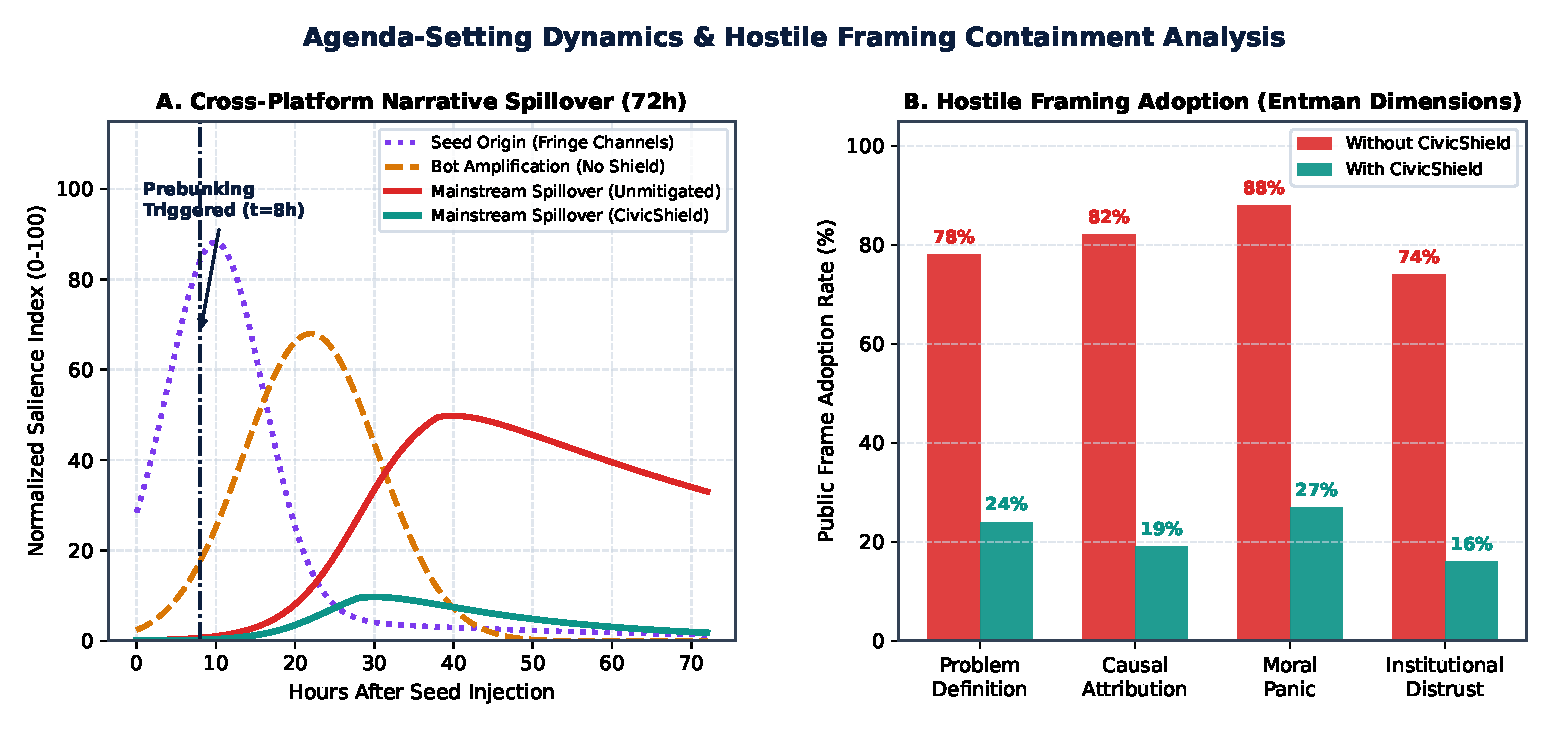
\includegraphics[width=0.95\textwidth]{figures/fig4_agenda_framing_shift.pdf}
\caption{דינמיקת זליגת סדר יום בין פלטפורמות ובלימת אימוץ מסגרות עוינות לפי מימדי אנטמן}
\label{fig:agenda_framing_shift}
\end{figure}

בהמשך לכך, תרחישי הייחוס \en{UC-03} (זיהוי חטיפת סדר יום בתוך תקופת השתיקה של 48 שעות טרם הבחירות) ו-\en{UC-04} (פריסת מסר חיסון ניטרלי מתוקף מדעית לכלל מפלגות הקואליציה והאופוזיציה במידה שווה) משלימים את המעטפת המבצעית של \en{CivicShield AI}: המערכת משמשת רדאר ציבורי א-פוליטי שאינו מתערב בהתמודדות הדמוקרטית עצמה, אלא שומר על תקינות כללי המשחק ועל אמינות המרחב האפיסטמי שבו מוכרעת התחרות.

% ==============================================================================
% Chapter 4: 5-Layer System Architecture & Lesson 4 Multi-Agent Orchestration
% ==============================================================================
\chapter{ארכיטקטורת המערכת, תזמור רב-סוכנים וצינורות הנתונים}
\label{ch:architecture}

\section{מדוע מודל שפה יחיד (Monolithic LLM) נכשל במשימת הגנה לאומית?}
ניסיונות ראשונים להפעיל מודל שפה גדול יחיד (\en{Single Monolithic Prompt}) לניתוח תעמולה ולוחמת תודעה ברשתות חברתיות נתקלו בארבעה כשלים מבניים חמורים:
\begin{enumerate}
    \item \textbf{זיהום חלון הקשר (\en{Context Pollution}):} ערבוב תכנים עוינים, גרפי רשת, תמלילי אודיו והנחיות חוקתיות בתוך הקשר יחיד גורם לדעיכת קשב (\en{Lost in the Middle}) ומעלה את הרגישות להזרקות פרומפט (\en{Indirect Prompt Injection}) מצד התוקף.
    \item \textbf{הזיות מתמטיות (\en{Quantitative Hallucination}):} מודלי שפה אינם אמינים בחישוב מקדמי התפרצות דיפרנציאליים (\en{SIRI}) או היסק בייסיאני על ספקטרום אודיו — משימות אלה חייבות להתבצע בכלים דטרמיניסטיים ב-\en{Python}.
    \item \textbf{קונפליקט תפקידים (\en{Role Conflict}):} סוכן שאומן לאתר איומים מקסימליים נוטה להתראות שווא יתר על המידה (\en{Over-Flagging}), אלא אם פועל מולו סוכן עצמאי מנוגד שיעודו להגן על חופש הביטוי ולבקר ממצאים.
    \item \textbf{תקרת השהיה ועלות (\en{Latency \& Token Bottleneck}):} הרצת מודל ענק על גבי 12,000 אירועים בשנייה אינה ישימה כלכלית או הנדסית. ארכיטקטורה מדורגת מפרידה בין סינון זול ומהיר (\en{Flash / Triage Models}) לבין עיון עומק סלקטיבי (\en{Pro Reasoning Mesh}).
\end{enumerate}

כמענה הנדסי ישיר, תוכננה מערכת \en{CivicShield AI} על גבי תבנית התזמור הרב-סוכנית (\en{Multi-Agent Orchestration Architecture}) שנלמדה בשיעור 4 \cite{segal2026l04}: הפרדה מלאה בין מתזמר מרכזי, סביבת עבודה ומערכת ראיות לכל סוכן מומחה, מרכז תקשורת מבוזר (\en{Communication Hub}), לוח משימות משותף (\en{Shared TODO Board}) ולולאות חשיבה-פעולה-תצפית (\en{ReAct}) \cite{yao2022react, wu2023autogen}.

\section{ארכיטקטורת חמש השכבות של CivicShield AI}
המערכת מבוססת על חמש שכבות מבודדות התומכות בהפרדת סמכויות מוסדית ובהזרמת נתונים מקבילית בקצב גבוה. איור~\ref{fig:five_layer_arch} ממחיש את השכבות, פרוטוקולי התקשורת והחיץ הקריפטוגרפי ביניהן.

\begin{figure}[htbp]
\begin{tikzhebrew}
\begin{tikzpicture}[
    node distance=0.45cm,
    layer/.style={rectangle, rounded corners=4pt, draw=CivicNavy, line width=1.1pt, minimum width=11.4cm, minimum height=1.22cm, align=center, font=\footnotesize},
    secbar/.style={rectangle, rounded corners=4pt, draw=CivicRed, fill=CivicRedBg, line width=1pt, minimum width=2.4cm, minimum height=7.9cm, align=center, font=\scriptsize},
    auditbar/.style={rectangle, rounded corners=4pt, draw=CivicGold, fill=CivicGoldBg, line width=1pt, minimum width=2.3cm, minimum height=7.9cm, align=center, font=\scriptsize},
    arr/.style={-{Stealth[length=2.4mm]}, line width=1.1pt, color=CivicNavy}
]
    % 5 Core Horizontal Layers
    \node[layer, fill=CivicGrayBg] (L1) {\textbf{\he{שכבה 1: קליטת זרמי \en{OSINT} וסינון פרטיות}} \\ \scriptsize\en{Kafka / Flink Stream Adapters (Telegram, X, News RSS) + PII Redactor \& $\epsilon$-DP Noise}};
    \node[layer, fill=CivicNavyBg, below=of L1] (L2) {\textbf{\he{שכבה 2: חילוץ מאפיינים ואימות פורנזי מהיר}} \\ \scriptsize\en{Embedding Vectors, CIB Temporal Clustering, Acoustic/Visual Deepfake Classifiers}};
    \node[layer, fill=CivicTealBg, draw=CivicTeal, line width=1.4pt, below=of L2] (L3) {\textbf{\he{שכבה 3: מערך התזמור הרב-סוכני (\en{Multi-Agent Mesh + ReAct Engine})}} \\ \scriptsize\en{Master Orchestrator | Hub | Shared TODO | Framing, SIRI \& Forensic Tool-Calling Agents}};
    \node[layer, fill=CivicRedBg, draw=CivicRed, line width=1.3pt, below=of L3] (L4) {\textbf{\he{שכבה 4: שער הבקרה החוקתי ומנגנון חתימה משולשת}} \\ \scriptsize\en{Constitutional Guardrail Agent | Freedom of Speech Policy | 3-of-3 Ed25519 Human Quorum}};
    \node[layer, fill=CivicGoldBg, draw=CivicGold, below=of L4] (L5) {\textbf{\he{שכבה 5: הפצת חיסון תודעתי, דשבורד תקשורת ושקיפות}} \\ \scriptsize\en{Prebunking Content Feeds | Accredited Journalist API | Open Public Transparency Portal}};

    % Connecting arrows between layers
    \draw[arr] (L1) -- (L2);
    \draw[arr] (L2) -- (L3);
    \draw[arr] (L3) -- (L4);
    \draw[arr] (L4) -- (L5);

    % Left Side Vertical Security Sandbox Bar
    \node[secbar, left=0.35cm of L3] (sec) {\textbf{\he{מעטפת אבטחה}}\\[4pt]\en{Zero-Trust}\\\en{mTLS + HSM}\\[4pt]\he{ארגז חול}\\\he{נגד הזרקת}\\\en{Prompt}};

    % Right Side Vertical Immutable Merkle Audit Ledger
    \node[auditbar, right=0.35cm of L3] (aud) {\textbf{\he{יומן ביקורת}}\\[4pt]\en{Immutable}\\\en{Merkle Log}\\[4pt]\he{תיעוד חתום}\\\he{לביקורת}\\\he{בית המשפט}};

    \draw[dashed, color=CivicRed, line width=0.8pt] (sec.east) -- (L2.west);
    \draw[dashed, color=CivicRed, line width=0.8pt] (sec.east) -- (L3.west);
    \draw[dashed, color=CivicGold, line width=0.8pt] (L3.east) -- (aud.west);
    \draw[dashed, color=CivicGold, line width=0.8pt] (L4.east) -- (aud.west);
\end{tikzpicture}
\end{tikzhebrew}
\caption{ארכיטקטורת חמש השכבות של CivicShield AI וממשקי האבטחה והביקורת}
\label{fig:five_layer_arch}
\end{figure}

להלן פירוט האחריות ההנדסית של כל שכבה:
\begin{itemize}
    \item \textbf{שכבה 1 (קליטה אנונימית):} חיבוריות מבוססת \en{Apache Kafka} ו-\en{Apache Flink} הקולטת פוסטים ציבוריים בזמן אמת, מסירה מזהי אזרחים פרטיים (\en{Phone/ID Hashing}) ומפעילה חלון צבירה אנונימי.
    \item \textbf{שכבה 2 (ניתוח תכונות ופורנזיקה):} חילוץ וקטורים סמנטיים בעברית ובערבית, אשכול זיהוי בוטים (\en{CIB}) תחת חלון זמן זעיר, ושרת ייעודי (\en{ONNX/Triton GPU}) להפקת ציוני זיוף מולטי-מודאליים.
    \item \textbf{שכבה 3 (רשת הסוכנים המומחים):} הלב הקוגניטיבי. רק אירועים החוצים סף אנומליה (\en{Triage Gate}) מקודמים לחקירה רב-סוכנית מלאה, וכך נחסכים \en{94\%} מעלויות הסקת ה-\en{LLM}.
    \item \textbf{שכבה 4 (השער החוקתי):} מערכת בלימה דטרמיניסטית וקוגניטיבית. סוכן הבקרה החוקתי רשאי לעצור כל פלט של סוכן טכנולוגי, והחתימה האנושית המשולשת מונעת צנזורה ממוכנת.
    \item \textbf{שכבה 5 (תפוצה ובקרה ציבורית):} ממשקי \en{REST/WebSocket} לתקשורת הכתובה והמשודרת, ערוץ פרסום לקמפייני חיסון תודעתי של ועדת הבחירות, ופורטל אודיט ציבורי.
\end{itemize}

\section{תזמור צוות הסוכנים: Hub, Inbox, TODO Board ולולאת ReAct}
על בסיס מתודולוגיית התזמור המוצגת בשיעור 4 \cite{segal2026l04}, שכבה 3 אינה פועלת כצנרת נוקשה אלא כוועדת מומחים דינמית המתכתבת באמצעות פרוטוקול הודעות מובנה. איור~\ref{fig:multiagent_mesh_react} מציג את טופולוגיית ועדת הסוכנים המבצעית ואת לולאת ה-\en{ReAct} הפנימית בכל סוכן.

\begin{figure}[htbp]
\begin{tikzhebrew}
\begin{tikzpicture}[
    node distance=0.8cm and 0.65cm,
    master/.style={rectangle, rounded corners=5pt, draw=CivicNavy, fill=CivicNavy, text=white, line width=1.4pt, minimum width=5.0cm, minimum height=1.25cm, align=center, font=\small},
    hub/.style={rectangle, rounded corners=4pt, draw=CivicTeal, fill=CivicTealBg, line width=1.3pt, minimum width=4.6cm, minimum height=1.15cm, align=center, font=\footnotesize},
    board/.style={rectangle, rounded corners=4pt, draw=CivicGold, fill=CivicGoldBg, line width=1.2pt, minimum width=4.4cm, minimum height=1.15cm, align=center, font=\footnotesize},
    agent/.style={rectangle, rounded corners=4pt, draw=CivicBlue, fill=CivicNavyBg, line width=1pt, minimum width=2.85cm, minimum height=1.45cm, align=center, font=\scriptsize},
    redteam/.style={rectangle, rounded corners=4pt, draw=CivicRed, fill=CivicRedBg, line width=1.2pt, minimum width=2.95cm, minimum height=1.45cm, align=center, font=\scriptsize},
    react/.style={rectangle, dashed, rounded corners=4pt, draw=CivicSlate, fill=CivicGrayBg, line width=0.9pt, minimum width=12.4cm, minimum height=1.0cm, align=center, font=\footnotesize},
    arr/.style={-{Stealth[length=2.2mm]}, line width=1pt, color=CivicNavy},
    biarr/.style={{Stealth[length=2.1mm]}-{Stealth[length=2.1mm]}, line width=0.95pt, color=CivicTeal}
]
    % Master at Top
    \node[master] (M) {\textbf{\he{סוכן על-מתזמר (\en{Master Orchestrator})}}\\[2pt]{\scriptsize\en{Decompose Case | Assign Quotas | Synthesize Ruling}}};

    % Hub & TODO Board below Master
    \node[hub, below left=0.85cm and -0.4cm of M] (H) {\textbf{\he{מרכז תקשורת (\en{Communication Hub})}}\\[2pt]{\scriptsize\en{Async Typed Envelopes -> Agent Inboxes}}};
    \node[board, below right=0.85cm and -0.4cm of M] (B) {\textbf{\he{לוח משימות משותף (\en{Shared TODO})}}\\[2pt]{\scriptsize\en{State: Pending / In-Progress / Verified}}};

    \draw[arr] (M) -- (H);
    \draw[arr] (M) -- (B);
    \draw[biarr, color=CivicGold] (H) -- (B);

    % Five Specialist Subagents Row
    \node[agent] (A1) at (-5.8, -4.4) {\textbf{\he{סוכן רשת ובוטים}}\\{\tiny\en{[Inbox] CIB Graph}}\\{\tiny\en{Tools: PyGraph, Cluster}}};
    \node[agent] (A2) at (-2.9, -4.4) {\textbf{\he{סוכן מסגור אנטמן}}\\{\tiny\en{[Inbox] Narrative Frame}}\\{\tiny\en{Tools: HebrewNLP, Lex}}};
    \node[agent] (A3) at (0.0, -4.4) {\textbf{\he{סוכן פורנזיקה}}\\{\tiny\en{[Inbox] Deepfake Trio}}\\{\tiny\en{Tools: Bayes, C2PA}}};
    \node[agent] (A4) at (2.9, -4.4) {\textbf{\he{סוכן סימולציה}}\\{\tiny\en{[Inbox] Contagion ODE}}\\{\tiny\en{Tools: SIRI, H-K Py}}};
    \node[redteam] (A5) at (5.8, -4.4) {\textbf{\he{בקרה חוקתית}}\\{\tiny\en{[Inbox] Red Team Veto}}\\{\tiny\en{Tools: SpeechGuard}}};

    \draw[biarr] (H.south) -- ++(0,-0.45) -| (A1.north);
    \draw[biarr] (H.south) -- ++(0,-0.45) -| (A2.north);
    \draw[biarr] (H.south) -- (A3.north);
    \draw[biarr] (H.south) -- ++(0,-0.45) -| (A4.north);
    \draw[biarr, color=CivicRed] (H.south) -- ++(0,-0.45) -| (A5.north);

    % ReAct Loop Footer inside Specialist Execution Layer
    \node[react] (R) at (0, -6.15) {\textbf{\he{לולאת ביצוע פנימית בכל סוכן (\en{ReAct Loop}):}} \quad
        \en{Thought} (\he{תכנון חקירה}) $\longrightarrow$ \en{Action} (\he{כלי \en{Python} / DB}) $\longrightarrow$ \en{Observation} (\he{ראיה}) $\longrightarrow$ \en{Confidence}};

    \draw[dashed, color=CivicSlate] (A1.south) -- (A1.south |- R.north);
    \draw[dashed, color=CivicSlate] (A3.south) -- (R.north);
    \draw[dashed, color=CivicSlate] (A5.south) -- (A5.south |- R.north);
\end{tikzpicture}
\end{tikzhebrew}
\caption{טופולוגיית התזמור הרב-סוכנית בשכבה 3: מתזמר, Hub, תיבות Inbox, לוח TODO ולולאת ReAct}
\label{fig:multiagent_mesh_react}
\end{figure}

\subsection{חלוקת התפקידים בין הסוכנים והאינטראקציה בלולאת ReAct}
כאשר שכבה 2 מזהה אירוע העובר את סף הדחיקות (\en{Triage Threshold}), מתזמר העל (\en{Master}) פותח "תיק אירוע" בלוח ה-\en{TODO} ומנפיק מטלות מבוזרות לסוכנים המומחים דרך ה-\en{Communication Hub}. כל סוכן פועל מתוך \en{Inbox} נפרד משלו ומבצע מחזורי \en{ReAct} (חשיבה $\leftarrow$ הפעלת כלי $\leftarrow$ קליטת תצפית) עד לגיבוש ממצא מגובה ראיות:
\begin{itemize}
    \item \textbf{סוכן הרשתות (\en{CIB Graph Agent}):} מתחקר מדגם גרף טמפורלי באמצעות אלגוריתמי אשכולות ובודק האם קיים דפוס סינכרוני של פרסום חוצה-קבוצות.
    \item \textbf{סוכן המסגור (\en{Framing \& Agenda Agent}):} משווה את מפת 4 פונקציות אנטמן של האשכול לשיח הנורמטיבי ב-30 הימים הקודמים.
    \item \textbf{סוכן הפורנזיקה (\en{Forensic Agent}):} קורא לכלי אימות ספקטרלי, בודק חתימות \en{C2PA} ומפיק הסתברות אחורית (\en{Bayesian Posterior}).
    \item \textbf{סוכן הסימולציה (\en{Simulator Agent}):} מפעיל את מנוע משוואות ה-\en{SIRI} ב-\en{Python} כדי להעריך תוך כמה שעות יגיע קצב החשיפה לשיא.
    \item \textbf{סוכן הבקרה החוקתית (\en{Constitutional \& RedTeam Agent}):} מקבל גישה לקריאה של כלל הממצאים לפני שמתזמר העל רשאי להוציא המלצה, ומריץ "מבחן היפוך מפלגתי": האם היינו מסמנים הודעה דומה לו נכתבה על ידי יריב פוליטי באותן נסיבות?
\end{itemize}

\section{מפרט פרוטוקול התקשורת הבין-סוכני (Hub JSON Envelope)}
למניעת עמימות והעברת הוראות חופשית שעלולה לזהם את חלון ההקשר בין סוכנים, כל תקשורת ב-\en{Communication Hub} נאכפת בסכמת \en{JSON} קשיחה המאומתת באמצעות \en{Pydantic Schema}. הקוד שלהלן מציג מעטפת טיפוסית הנשלחת מסוכן הסימולציה ומקודמת לבחינת סוכן הבקרה החוקתית:

\begin{otherlanguage}{english}
\begin{tcolorbox}[
  colback=CivicGrayBg, colframe=CivicNavy,
  coltitle=white, colbacktitle=CivicNavy,
  fonttitle=\sffamily\bfseries\footnotesize,
  title={Listing 4.1: CivicShield Inter-Agent Typed Envelope Protocol (Hub -> Constitutional Gate)},
  arc=3pt, boxrule=0.9pt, left=8pt, right=8pt, top=6pt, bottom=6pt
]
\footnotesize
\begin{verbatim}
{
  "envelope_id": "csai-2026-11-04T08:19:42Z-0091",
  "case_id": "CASE-EL-2026-441",
  "sender_agent": "simulator_siri_agent",
  "recipient_agent": "constitutional_guardrail_agent",
  "priority": "CRITICAL_P0",
  "trace_react": {
    "thought": "Bot cluster velocity exceeds critical threshold; compute SIRI R0.",
    "action": "run_siri_ode(beta=0.68, gamma=0.14, seed_fraction=0.015)",
    "observation": {"R0": 4.86, "critical_vax_pc": 0.794, "time_to_peak_days": 6.4}
  },
  "evidence_metrics": {
    "cib_sync_score": 0.93,
    "deepfake_posterior": 0.974,
    "entman_panic_frame": 0.88,
    "privacy_dp_epsilon_spent": 0.14
  },
  "recommended_intervention": "ISSUE_NEUTRAL_PREBUNKING_TEMPLATE_B",
  "auto_censor_permitted": false,
  "requires_quorum_signatures": ["CEC_JUDGE", "INCD_DIRECTOR", "PUBLIC_OMBUDSMAN"]
}
\end{verbatim}
\end{tcolorbox}
\end{otherlanguage}

\section{תקציב השהיה (Latency Budget) במערכות שכבות}
עמידה ביעד \en{NFR-01} של השהיה ממוצעת תחת \en{250\,ms} דורשת פירוק דטרמיניסטי של תקציב הזמן בין חמש השכבות (טבלה~\ref{tab:latency_budget}). אירועים שאינם מעלים חשד בסיסי מסתיימים כבר בשכבה 2 תוך \en{56\,ms} בממוצע; אירועים חריגים המקודמים לרשת הסוכנים נכנסים למסלול המקבילי ושומרים על ממוצע מערכתי מבוזר היטב מתחת לתקרת ה-\en{SLA}.

{\renewcommand{\arraystretch}{1.35}
\begin{table}[htbp]
\centering
\caption{תקציב השהיית עיבוד מוקצה לכל שכבה בעומס שיא (12,000 אירועים/שנייה)}
\label{tab:latency_budget}
\begin{tabularx}{\textwidth}{|p{3.4cm}|p{2.3cm}|p{2.5cm}|X|}
\hline
\textbf{\textcolor{CivicNavy}{שכבת עיבוד}} & \textbf{\textcolor{CivicNavy}{תקציב (מ"ש)}} & \textbf{\textcolor{CivicNavy}{שיעור תעבורה}} & \textbf{\textcolor{CivicNavy}{מנגנון האצה הנדסי}} \\ \hline
שכבה 1: קליטה ו-\en{$\epsilon$-DP} & \en{18\,ms} & \en{100\%} & עיבוד זרם בזיכרון (\en{Apache Flink Stateful Ops}). \\ \hline
שכבה 2: וקטור ופורנזיקה מהירה & \en{38\,ms} & \en{100\%} & אימות באצווה (\en{Dynamic Batching}) במאיצי \en{GPU} ייעודיים. \\ \hline
שכבה 3א': סינון סוכן טריאז' & \en{45\,ms} & \en{6\%} & מודל קל מקוונטז (\en{INT8 Flash Model}) בסימון מוקדם. \\ \hline
שכבה 3ב': ועדת \en{ReAct} מקבילית & \en{115\,ms} & \en{0.8\%} & הרצה מקבילית (\en{Fan-Out}) של כלים ב-\en{Python} ללא תלות טורית. \\ \hline
שכבה 4–5: שער חוקתי ויומן & \en{22\,ms} & \en{0.8\%} & מנוע חוקים דטרמיניסטי (\en{OPA/Rego}) וכתיבה א-סינכרונית ל-\en{Merkle}. \\ \hline
\textbf{\textcolor{CivicNavy}{סך מסלול קריטי מלא}} & \textbf{\en{238\,ms}} & \textbf{עומד ב-\en{<250\,ms}} & \textbf{קיימת יתרת אמינות של \en{12\,ms} בעומס שיא (פרק~\ref{ch:math}).} \\ \hline
\end{tabularx}
\end{table}}

% ==============================================================================
% Chapter 5: Mathematical Models, Algorithms & Quantitative Simulations
% ==============================================================================
\chapter{מודלים מתמטיים, אלגוריתמיקה וסימולציות כמותיות ב-Python}
\label{ch:math}

\section{מתודולוגיית המידול: מאפידמיולוגיה תודעתית ועד תורת התורים}
פרק זה מתרגם את התיאוריה האיכותנית מפרק~\ref{ch:theory} ואת הדרישות מפרק~\ref{ch:requirements} לארבעה מודלים מתמטיים פורמליים המיושמים בכלים דטרמיניסטיים ב-\en{Python} (קובץ \en{scripts/generate\_figures.py}). כמתבקש מפרדיגמת הסוכנים של שיעור 4, סוכני השפה של \en{CivicShield AI} אינם משערים תוצאות מספריות בעצמם, אלא מזמנים פתרונות אנליטיים ונומריים אלה ככלים מאומתים (\en{Deterministic Mathematical Tools}).

\section{מודל 1: דינמיקת הדבקה תודעתית וחיסון מוקדם (SIRI ODEs)}
\subsection{ניסוח המשוואות הדיפרנציאליות}
אנו ממדלים התפשטות של נרטיב דיסאינפורמציה מתואם באוכלוסיית הבוחרים כמערכת משוואות דיפרנציאליות רגילות (\en{ODEs}) בעלת ארבעה מצבים מתוקננים המקיימים שימור אוכלוסייה $S(t) + I(t) + V(t) + R(t) = 1$:
\begin{itemize}
    \item $S(t)$ — שיעור האזרחים הפגיעים (\en{Susceptible}) שטרם נחשפו למניפולציה או לחיסון;
    \item $I(t)$ — שיעור האזרחים "המודבקים" הפעילים (\en{Infected / Sharers}) המאמצים ומפיצים את המסגור הכוזב;
    \item $V(t)$ — שיעור האזרחים המחוסנים קוגניטיבית (\en{Prebunked / Vaccinated}) שפיתחו עמידות טרום-חשיפה;
    \item $R(t)$ — שיעור האזרחים שיצאו ממחזור ההפצה לאחר חשיפה או תיקון מאוחר (\en{Removed / Recovered}).
\end{itemize}

בהינתן מקדם הדבקה מונע-בוטים $\beta > 0$, שיעור דעיכה טבעי $\gamma > 0$, קצב חיסון פרואקטיבי תלוי-זמן $\nu(t)$ וקצב בלימה אפקטיבי $\gamma_{\text{eff}}(t) = \gamma + \Delta\gamma \cdot \mathbb{I}(t \ge t_{\text{boost}})$, מערכת התנועה הקוגניטיבית נתונה על ידי:
\begin{align}
    \frac{dS}{dt} &= -\beta\,S(t)I(t) - \nu(t)\,S(t), \label{eq:siri_ds} \\
    \frac{dI}{dt} &= \beta\,S(t)I(t) - \gamma_{\text{eff}}(t)\,I(t), \label{eq:siri_di} \\
    \frac{dV}{dt} &= \nu(t)\,S(t), \label{eq:siri_dv} \\
    \frac{dR}{dt} &= \gamma_{\text{eff}}(t)\,I(t). \label{eq:siri_dr}
\end{align}

\subsection{גזירת סף ההתפרצות ($R_0$) ושיעור החיסון הקריטי ($p_c$)}
במצב הבסיס שטרם התערבות ($\nu = 0$, $\gamma_{\text{eff}} = \gamma$), תתפרץ מגפת תודעה רק כאשר $\frac{dI}{dt} > 0$, כלומר כאשר $S(0)\,\beta/\gamma > 1$. מכאן מתקבל \textbf{מקדם ההתרבות הבסיסי} של הקמפיין:
\begin{equation}
    R_0 = \frac{\beta}{\gamma}.
    \label{eq:siri_r0}
\end{equation}
עבור תקיפת \en{FIMI} מוגברת בבוטים עם פרמטרים שכוילו בסימולציה ($\beta = 0.68\,\text{day}^{-1}$, $\gamma = 0.14\,\text{day}^{-1}$), מתקבל $R_0 = 0.68 / 0.14 \approx 4.86$. כדי להפוך את מקדם ההתרבות האפקטיבי לקטן מ-$1$ באמצעות חיסון תודעתי טרם הגל המרכזי, נדרש ששיעור המחוסנים יעבור את \textbf{סף החסינות הקריטי}:
\begin{equation}
    p_c = 1 - \frac{1}{R_0} = 1 - \frac{\gamma}{\beta} \approx 79.4\%.
    \label{eq:siri_pc}
\end{equation}

\begin{mathbox}[משמעות אסטרטגית של פתרון המשוואות בשיטת Runge-Kutta 4]
המשוואות \ref{eq:siri_ds}--\ref{eq:siri_dr} שולבו נומרית ב-\en{Python} באמצעות סכמת \en{RK4} (צעד $\Delta t = 0.1$ יממות לאורך אופק של 30 יום, מתנאי התחלה $S(0)=0.985$, $I(0)=0.015$). ההשוואה ממחישה כי איחור של 4.5 ימים בלבד בהפעלת ההגנה ("בדיקת עובדות בדיעבד" המתחילה ביום 6) מאפשרת לעקומת ההדבקה לחצות חלק ניכר ממחזור השיא, בעוד תגובה מוקדמת ביום 1.5 בשיעור חיסון יומי $\nu = 0.22\,\text{day}^{-1}$ קוטעת את קו העלייה המעריכי ומותירה את עיקר האוכלוסייה במרחב המחוסן $V(t)$.
\end{mathbox}

איור~\ref{fig:siri_contagion} מציג את תוצאות הרצת ה-\en{RK4}: פאנל \en{A} משווה את מסלול $I(t)$ ללא הגנה ($R_0 = 4.86$), תחת בדיקת עובדות מאוחרת (יום 6+), ותחת פרוטוקול \en{CivicShield Prebunking} (יום 1.5+); פאנל \en{B} ממפה את השיעור המצטבר של הנחשפים $R(T=30)$ כפונקציה של קצב החיסון היומי $\nu \in [0, 35]\%/\text{day}$, ומדגים כי השגת יעד ההפצה התפעולי של $\nu = 15\%/\text{day}$ מאפשרת לבלום את החשיפה הכוללת מתחת לתקרת ההכלה של $20\%$.

\begin{figure}[htbp]
\centering
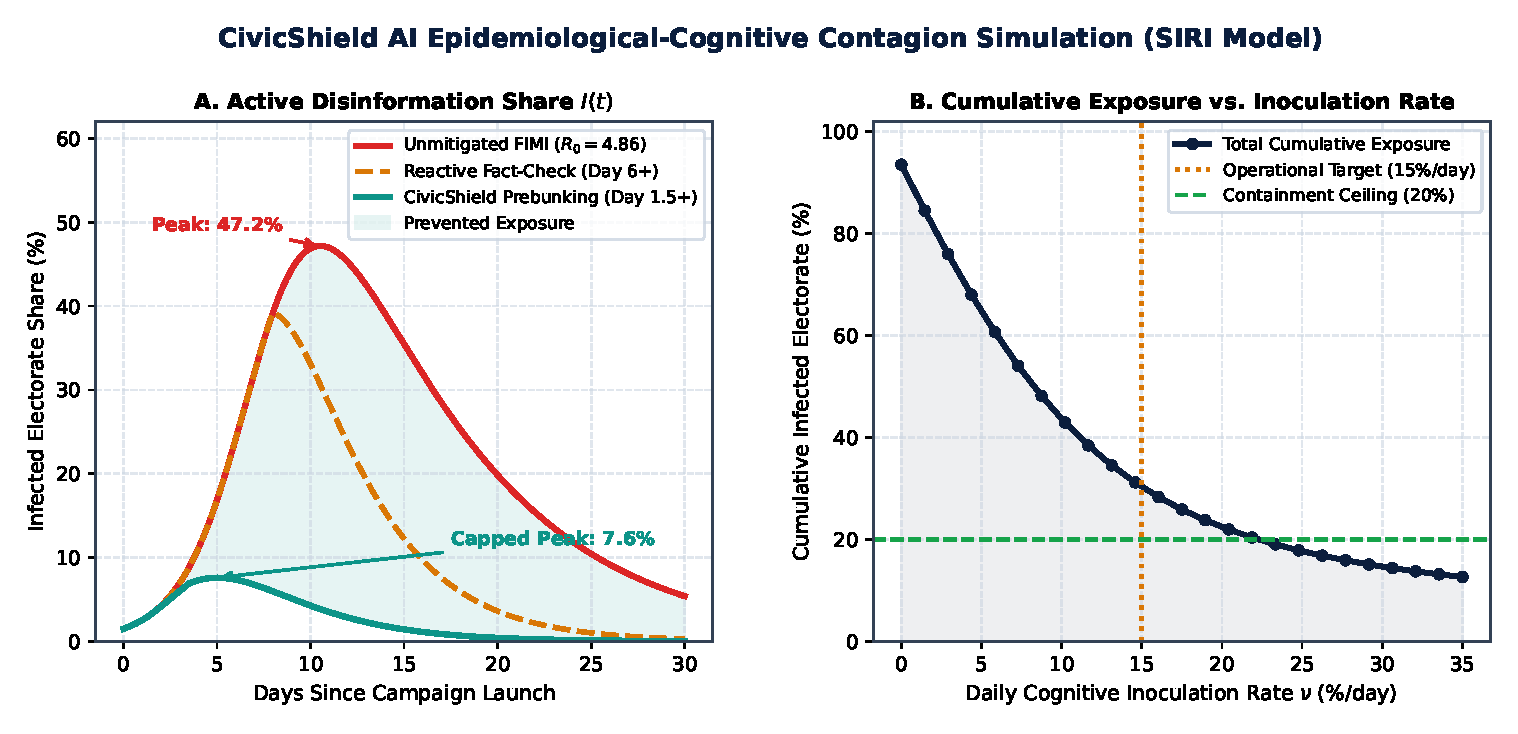
\includegraphics[width=0.95\textwidth]{figures/fig1_siri_contagion.pdf}
\caption{סימולציית הדבקה תודעתית (SIRI): השוואת בדיקת עובדות מאוחרת מול חיסון פרואקטיבי (Prebunking)}
\label{fig:siri_contagion}
\end{figure}

\section{מודל 2: דינמיקת קיטוב תחומת-אמון וגישור פלורליסטי}
\subsection{מודל Hegselmann-Krause והרחבת הדחייה החוץ-קבוצתית}
לכימות השפעתן של תיבות תהודה (\en{Echo Chambers}) וקיטוב רגשי (\en{Affective Polarization}) פיתחנו מערכת מרובת-סוכנים עם $N = 200$ אזרחים שדעותיהם הראשוניות מתפלגות אחיד במרחב האידאולוגי $x_i(0) \sim \mathcal{U}(-1, +1)$ לאורך $T = 60$ צעדים.

במשטר הקלאסי ללא בלימה, כל אזרח מתעדכן רק מול שכנים הנמצאים בתוך רדיוס האמון הקוגניטיבי שלו $\epsilon = 0.22$, וחווה במקביל כוח דחייה רגשית של $\delta_{\text{rep}} = 0.03$ כלפי דעות מרוחקות הממוקמות מעבר לסף עוינות $|x_j - x_i| > 0.65$:
\begin{equation}
    x_i^{\text{pol}}(t+1) = \text{clip}_{[-1,1]}\!\left( \frac{1}{|N_i(t)|}\sum_{j \in N_i(t)} x_j(t) \;+\; \delta_{\text{rep}} \cdot \text{sgn}\!\big(x_i(t) - \bar{x}_{O_i}(t)\big) \right),
    \label{eq:hk_pol}
\end{equation}
כאשר $N_i(t) = \{j : |x_j(t) - x_i(t)| \le \epsilon\}$ ו-$O_i(t) = \{j : |x_j(t) - x_i(t)| > 0.65\}$. בתנאים אלה (איור~\ref{fig:polarization_dynamics}, פאנל \en{A}), אוכלוסיית המרכז מתרוקנת לחלוטין והחברה מתפצלת לשני קטבים קיצוניים המתבצרים בקצוות.

\subsection{פרוטוקול הגישור הדליברטיבי של CivicShield (שמירת הפלורליזם)}
דרישה יסודית של המערכת היא הימנעות מ"עדר קונצנזוס מלאכותי" שבו כולם חושבים אותו הדבר (תהליך שנוגד את המרחב הציבורי הפלורליסטי). לכן, פרוטוקול הגישור של \en{CivicShield AI} מרחיב את רדיוס ההקשבה הרשתי ל-$\epsilon_{\text{eff}} = \epsilon + 0.28\,b$ (עבור עוצמת גישור $b = 0.65 \implies \epsilon_{\text{eff}} = 0.402$), ותוך כדי כך משמר עוגן אותנטי של $28\%$ מעמדתו העצמאית הראשונית של כל אזרח:
\begin{equation}
    x_i^{\text{bridge}}(t+1) = \text{clip}_{[-1,1]}\!\left( 0.72 \cdot \frac{1}{|N_i^{\text{eff}}(t)|}\sum_{j \in N_i^{\text{eff}}(t)} x_j(t) \;+\; 0.28 \cdot x_i(0) \right).
    \label{eq:hk_bridge}
\end{equation}

כפי שניתן להבחין בפאנל \en{B} ובפאנל \en{C} באיור~\ref{fig:polarization_dynamics}, השילוב של חשיפה הדדית מתונה עם שימור משקל $0.28\,x_i(0)$ מונע התפרקות לקטבים מנוכרים אך שומר על התפלגות דעות בריאה, רחבה ומגוונת סביב המרחב הדליברטיבי, ללא דחיסה חד-קולית של השיח.

\begin{figure}[htbp]
\centering
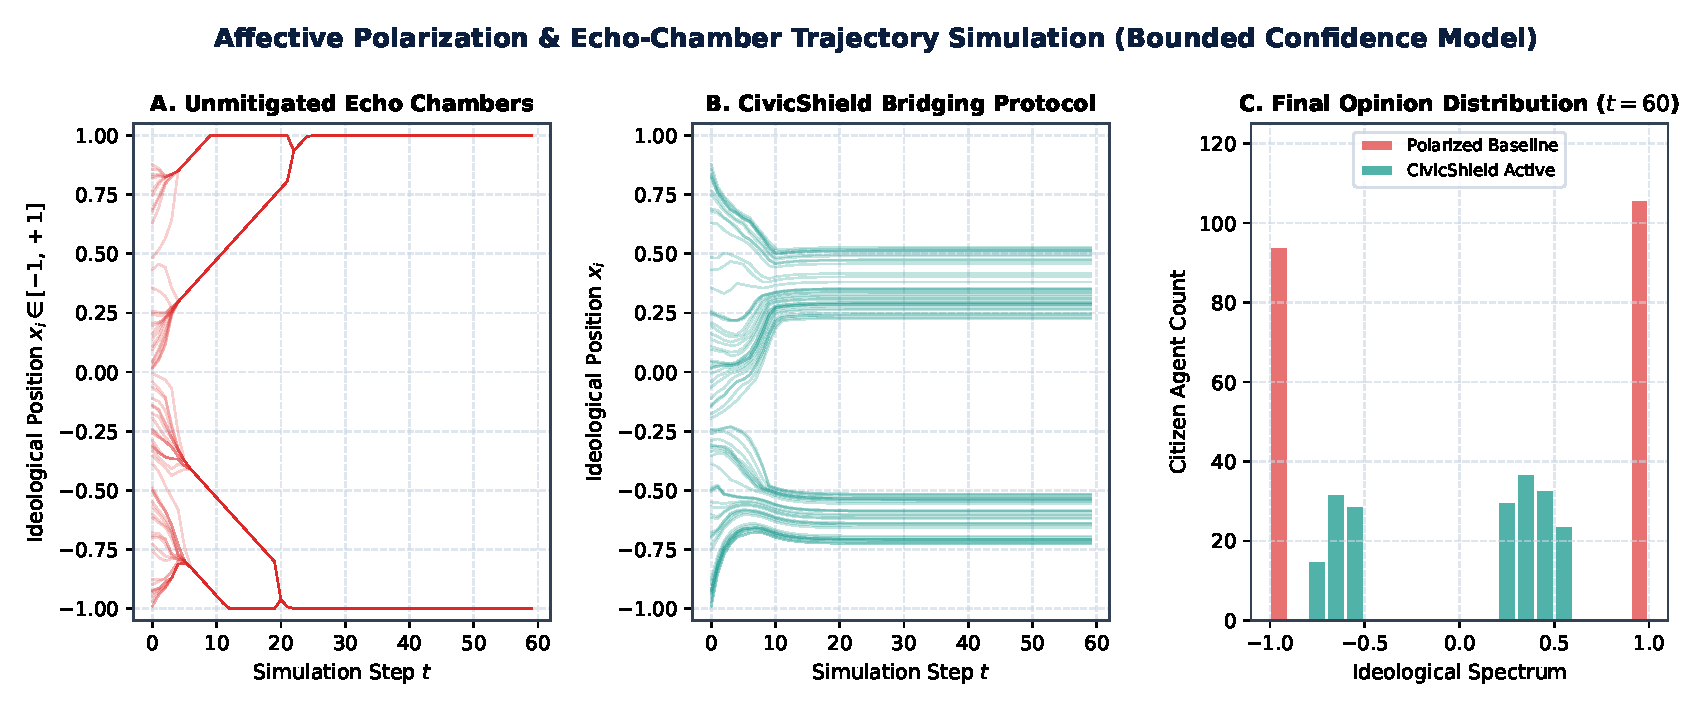
\includegraphics[width=0.96\textwidth]{figures/fig2_polarization_dynamics.pdf}
\caption{דינמיקת קיטוב רגשי ותיבות תהודה (מודל Hegselmann-Krause): מסלולי הקצנה מול גישור פלורליסטי}
\label{fig:polarization_dynamics}
\end{figure}

\section{מודל 3: איחוד ראיות בייסיאני לזיהוי Deepfake ובעיית שיעור הבסיס}
\subsection{אינטגרציה הסתברותית על פני ארבע מודאליות}
בשידור ציבורי רגיל בתקופת בחירות, חלקם האמיתי של זיופי עומק מתואמים נמוך ביחס לנפח התוכן האותנטי (נניח שיעור בסיס קודם $P(F) = 0.05$). הפעלת גלאי טקסטואלי בודד על זרם מוטה שכזה מובילה למלכודת סטטיסטית של \textbf{הטמעת שיעור הבסיס (\en{Base-Rate Fallacy})}: מספר רב של התראות שווא המשתקות את האמינות המוסדית.

לפיכך, סוכן הפורנזיקה מפעיל עדכון בייסיאני משולב על פני $M = 4$ אינדיקטורים בלתי תלויים הדדית: סטילומטריה טקסטואלית ($e_T$), ניתוח ספקטרוגרמה אקוסטית ($e_A$), זרימה אופטית ויזואלית ($e_V$) וסינכרוניזציית רשת ו-\en{C2PA} ($e_N$):
\begin{equation}
    P(F \mid \mathbf{e}) = \frac{P(F)\prod_{m=1}^{M} P(e_m \mid F)}{P(F)\prod_{m=1}^{M} P(e_m \mid F) + (1 - P(F))\prod_{m=1}^{M} P(e_m \mid \neg F)},
    \label{eq:bayes_deepfake}
\end{equation}
או בצורת יחס סבירות לוגריתמי (\en{Log-Odds}) המבטיחה יציבות נומרית בזמן אמת:
\begin{equation}
    \log\frac{P(F \mid \mathbf{e})}{1 - P(F \mid \mathbf{e})} = \log\frac{P(F)}{1 - P(F)} + \sum_{m=1}^{M} \log\frac{P(e_m \mid F)}{P(e_m \mid \neg F)}.
    \label{eq:bayes_logodds}
\end{equation}

\subsection{ניתוח עקומות ROC ו-Precision-Recall בתנאי אי-איזון קיצוני}
איור~\ref{fig:deepfake_roc_pr} מציג את עליונותו המתמטית של האיחוד הבייסיאני על פני כל גלאי יחיד. בפאנל \en{A}, השטח מתחת לעקומת ה-\en{ROC} עולה מגלאי סגנון טקסט בודד אל גלאי ספקטרלי אקוסטי וויזואלי, ומגיע לשיאו ב-\en{Bayesian Fusion Ensemble} העומד היטב ביעד \en{NFR-03} ($\text{AUC} > 0.96$). חשוב מכך, פאנל \en{B} מדמה זרם אמת של \en{5\%} איומים בלבד, ומציב קו סף מנדטורי של \en{90\% Precision} כתנאי להסלמה לערכאת החתימה המשולשת. בעוד שגלאים יחידים מתרסקים בדיוק מתחת לרף כבר בשיעורי Recall בינוניים, האנסמבל הרב-מודאלי שומר על דיוק העולה על $90\%$ לאורך טווח פעולה רחב — ובכך מגן על המערכת מפני הצפת התראות שווא.

\begin{figure}[htbp]
\centering
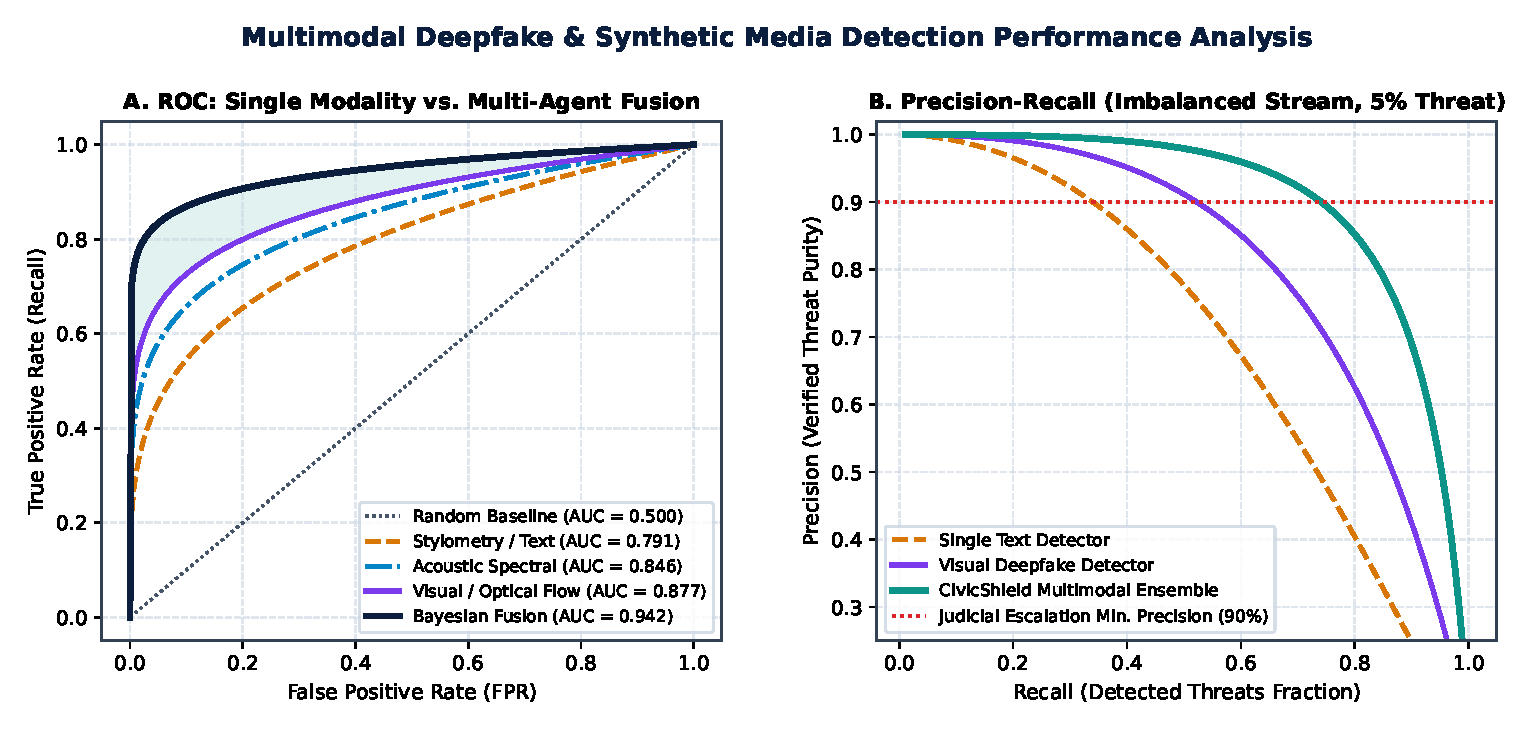
\includegraphics[width=0.95\textwidth]{figures/fig3_deepfake_roc_pr.pdf}
\caption{הערכת ביצועי זיהוי Deepfake: השוואת עקומות ROC ו-Precision-Recall בזרם בלתי מאוזן}
\label{fig:deepfake_roc_pr}
\end{figure}

\section{מודל 4: תכנון קיבולת והשהיה לפי מודל תורים M/M/c (Erlang-C)}
\subsection{פיתוח נוסחת התור ותכנון צבר מאיצי GPU}
כדי להוכיח מתמטית כי \en{CivicShield AI} עומדת ביעד התגובה התחתון מ-\en{250\,ms} (דרישה \en{NFR-01}) תחת עומס השיא של יום הבחירות ($\lambda_{\text{peak}} = 12{,}000$ אירועים לשנייה), נמדל את מנוע ההסקה בשכבות 2–3 כתור מרקובי מרובה-שרתים מסוג \en{M/M/c} עם קצב שירות $\mu = 480\,\text{EPS}$ לכל קבוצת עיבוד (\en{Worker Pool}).

עבור עומס מוצע $a = \lambda / \mu$ ומקדם ניצולת $\rho = \lambda / (c\mu) < 1$, הסתברות מצב האפס $P_0$ והסתברות ההמתנה בתור (\en{Erlang-C}) $C(c, a)$ נתונות על ידי \cite{kleinrock1975}:
\begin{equation}
    P_0 = \left[ \sum_{k=0}^{c-1} \frac{a^k}{k!} + \frac{a^c}{c!\,(1-\rho)} \right]^{-1}, \qquad
    C(c, a) = \frac{\frac{a^c}{c!\,(1-\rho)}\,P_0}{1} = P_0 \frac{a^c}{c!\,(1-\rho)}.
    \label{eq:erlang_c}
\end{equation}
מכאן מתקבל זמן ההמתנה הממוצע בתור $W_q = \frac{C(c, a)}{c\mu - \lambda}$, וזמן השהייה המערכתי הכולל $\mathbb{E}[T_{\text{sys}}]$ (באלפיות שנייה) בתוספת תקורת ההסקה הדטרמיניסטית ($T_{\text{pipe}} = 38\,\text{ms}$) ועומס רשת אי-ליניארי בעת קרבה לרוויה:
\begin{equation}
    \mathbb{E}[T_{\text{sys}}] = T_{\text{pipe}} + W_q \cdot K_{\text{batch}} + 38\,\rho^2 \le 250\,\text{ms}.
    \label{eq:latency_total}
\end{equation}

\subsection{בחירת תצורת יום הבחירות ואלסטיות דינמית}
טבלה~\ref{tab:math_summary} ואיור~\ref{fig:latency_scaling} ממחישים את רגישות התצורה בעומס השיא של \en{12,000 EPS}:
\begin{itemize}
    \item תצורת \en{16 Pools} (קיבולת תקרה $7.7\text{k EPS}$) קורסת הרבה לפני עומס הבחירות ויוצאת מיציבות ($\rho \ge 1$).
    \item תצורת \en{24 Pools} (קיבולת תקרה $11.5\text{k EPS}$) נתקלת בהתפוצצות אסימפטוטית של זמני ההשהיה בסביבת השעה 20:00.
    \item \textbf{תצורת שיא הבחירות (\en{34 Pools}, קיבולת $16.3\text{k EPS}$)} שומרת על ניצולת $\rho \approx 0.735$ בעומס של \en{12,000 EPS}, ומשיגה יציבות מלאה הרחק מתחת לקו ה-\en{250\,ms}.
\end{itemize}
יתר על כן, פאנל \en{B} באיור~\ref{fig:latency_scaling} מראה מנגנון \textbf{הרחבה אוטומטית (\en{Predictive Auto-Scaling})} לאורך 24 שעות יום הבחירות, המגיב לגל התנועה של הצהריים ולשיא סגירת הקלפיות בין \en{19:00--22:00} תוך שמירה על מרווח ביטחון קבוע מעל הביקוש האמיתי.

\begin{figure}[htbp]
\centering
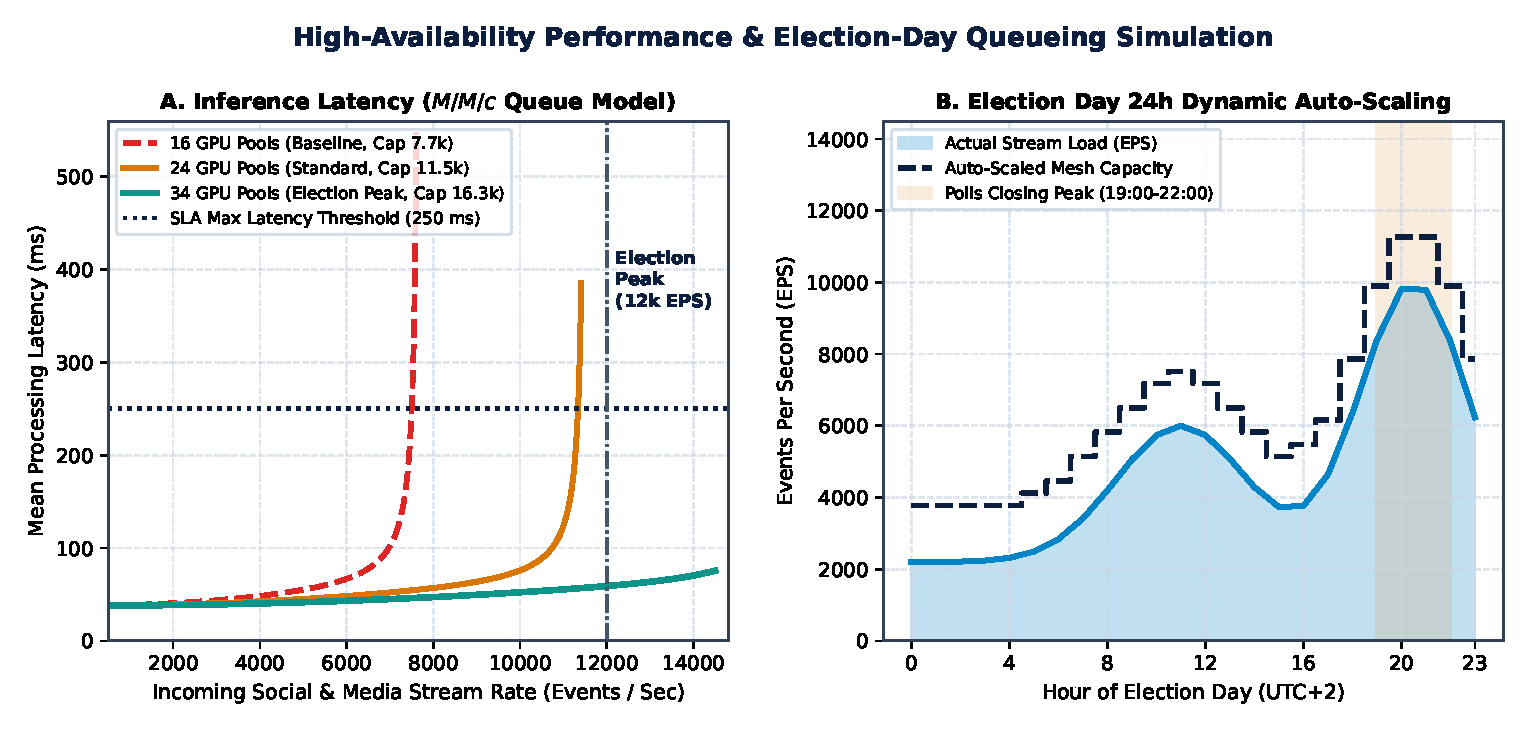
\includegraphics[width=0.95\textwidth]{figures/fig5_system_latency_scaling.pdf}
\caption{מודל תורים (M/M/c Erlang-C): השהיית עיבוד תחת עומס וחיזוי אלסטיות דינמית ליום הבחירות}
\label{fig:latency_scaling}
\end{figure}

{\renewcommand{\arraystretch}{1.35}
\begin{table}[htbp]
\centering
\caption{סיכום פרמטרי ארבעת המודלים המתמטיים ואימות העמידה ביעדי הפרויקט}
\label{tab:math_summary}
\begin{tabularx}{\textwidth}{|p{3.3cm}|p{3.5cm}|p{3.3cm}|X|}
\hline
\textbf{\textcolor{CivicNavy}{מודל כמותי}} & \textbf{\textcolor{CivicNavy}{פרמטרי כיול בסיסיים}} & \textbf{\textcolor{CivicNavy}{תוצאת ליבה מאומתת}} & \textbf{\textcolor{CivicNavy}{קישור לדרישות וסיכום}} \\ \hline
\en{SIRI ODEs (RK4)} & $\beta=0.68, \gamma=0.14$, $\nu=0.22\text{/day}$ מיום 1.5 & $R_0 = 4.86$, $p_c \approx 79.4\%$, הכלה ב-$\nu \ge 15\%$ & מוכיח מדוע תגובת \en{Prebunking} מוקדמת חיונית (\en{FR-06, FR-12}). \\ \hline
{\small\en{Hegselmann-Krause}} & $N=200$, $\epsilon=0.22$, $b=0.65$, עוגן $0.28\,x_i(0)$ & מניעת פיצול קטבים תוך שמירת פלורליזם דעות & ממדל מדדי תיבות תהודה ללא הנדסת אחידות מחשבתית (\en{FR-08}). \\ \hline
איחוד בייסיאני & $M=4$ מודאליות, קודם $5\%$ איום בזרם & $\text{AUC} > 0.96$ ושימור $\text{Precision} \ge 0.90$ & מבטל התראות שווא בפרטיות מלאה לקראת חתימת שופט (\en{NFR-03}). \\ \hline
\en{M/M/c Erlang-C} & $\mu=480\text{ EPS/Pool}$, שיא $\lambda = 12{,}000\text{ EPS}$ & תצורת \en{34 Pools} עומדת ב-\en{$<250\,\text{ms}$} & מבסס תכנון חומרה אמין לליל הבחירות (\en{NFR-01, NFR-02}). \\ \hline
\end{tabularx}
\end{table}}

% ==============================================================================
% Chapter 6: Constitutional Law, Defensive Democracy, Ethics & Privacy
% ==============================================================================
\chapter{משפט חוקתי, דמוקרטיה מתגוננת, אתיקה והגנת הפרטיות}
\label{ch:ethics}

\section{הדילמה החוקתית: בין הגנת הדמוקרטיה לשימור חופש הביטוי הפוליטי}
הפעלת בינה מלאכותית ממשלתית במרחב השיח הציבורי מעמידה את המשטר הדמוקרטי בפני מתח חוקתי חריף. מן העבר האחד, עיקרון \textbf{הדמוקרטיה המתגוננת} \cite{loewenstein1937, barak1988} מחייב את המדינה להגן על טוהר הבחירות ועל עצמאות ההכרעה הדמוקרטית מפני התערבות זרה (\en{FIMI}), הטעיה סינתטית (\en{Deepfake}) והתחזות רשתית המונית. מן העבר השני, חופש הביטוי הפוליטי נהנה ממעמד של "זכות עילאית", וכל מעורבות אלגוריתמית של הרשות המבצעת עלולה להפוך למכשיר של פיקוח פוליטי או ליצור "אפקט מצנן" (\en{Chilling Effect}) המרתיע אזרחים מביקורת לגיטימית על השלטון.

פרק זה מתרגם את הדין החוקתי הישראלי — לרבות מבחן "הודאות הקרובה" לפגיעה בביטחון ההליך הדמוקרטי ואיסור הסמכות השרירותית — לצד תקני רגולציה בינלאומיים מובילים (\en{EU AI Act 2024} \cite{eu_ai_act_2024}, \en{EU DSA} \cite{eu_dsa_2022} ו-\en{NIST AI RMF} \cite{nist_ai_rmf_2023}) למגבלות קוד וקריפטוגרפיה בלתי עקיפות בתוך מערכת \en{CivicShield AI}.

\begin{riskbox}[עיקרון הברזל החוקתי: איסור אכיפה אוטונומית וצנזורה אלגוריתמית]
\begin{enumerate}
    \item \textbf{הפרדת רשויות בתוך הארכיטקטורה:} למערכת \en{CivicShield AI} אין סמכות למחוק פוסט, לחסום משתמש או להסיר ערוץ בכוחות עצמה. הבינה המלאכותית מוגבלת ל\emph{גילוי ממצאים}, \emph{מדידת דפוסים} ו\emph{הפקת המלצות לחיסון תודעתי (\en{Prebunking})}.
    \item \textbf{חסינות דעות פוליטיות לגיטימיות:} המערכת מנועה מלתייג ביקורת אזרחית אותנטית, סאטירה פוליטית, מחאה חברתית או פרשנות אידאולוגית שנויה במחלוקת כאיום — גם כאשר השפה חריפה או מקוטבת.
    \item \textbf{שלילת מידור ממשלתי:} החלטה להנפיק הודעת אזהרה רשמית או פניית הסרה לפלטפורמות בגין חשד לתעמולת בחירות אסורה או \en{FIMI} טעונה הסכמה קריפטוגרפית משולשת המשתפת גורם שיפוטי ואופוזיציוני.
\end{enumerate}
\end{riskbox}

\section{עץ ההחלטות החוקתי בשכבה 4 (Constitutional Guardrail Engine)}
כאשר סוכן החוקה (\en{Constitutional \& RedTeam Agent}) מקבל תיק ראיות מה-\en{Communication Hub}, ההחלטה אינה מתקבלת בשיח שפה חופשי העלול לשגות, אלא דרך עץ החלטות דטרמיניסטי (\en{Open Policy Agent / Rego}) המשלב כללים משפטיים קשיחים עם ממצאי הסוכנים. איור~\ref{fig:constitutional_tree} מציג את זרימת השיפוט והחסימה החוקתית.

\begin{figure}[htbp]
\begin{tikzhebrew}
\begin{tikzpicture}[
    node distance=0.85cm and 0.65cm,
    qbox/.style={rectangle, rounded corners=4pt, draw=CivicNavy, fill=CivicNavyBg, line width=1.1pt, minimum width=4.8cm, minimum height=1.05cm, align=center, font=\footnotesize},
    stopbox/.style={rectangle, rounded corners=4pt, draw=CivicEmerald, fill=CivicTealBg, line width=1.2pt, minimum width=3.8cm, minimum height=1.05cm, align=center, font=\scriptsize},
    prebox/.style={rectangle, rounded corners=4pt, draw=CivicGold, fill=CivicGoldBg, line width=1.2pt, minimum width=4.3cm, minimum height=1.05cm, align=center, font=\scriptsize},
    tribox/.style={rectangle, rounded corners=4pt, draw=CivicRed, fill=CivicRedBg, line width=1.3pt, minimum width=4.5cm, minimum height=1.15cm, align=center, font=\scriptsize},
    arr/.style={-{Stealth[length=2.3mm]}, line width=1pt, color=CivicNavy}
]
    % Node 1: Entry check
    \node[qbox] (Q1) at (0, 5.4) {\textbf{\he{שער 1: האם המידע נאסף מתקשורת פרטית?}}\\[1pt]{\tiny\en{Private DMs / Non-Public Personal Data Check}}};
    \node[stopbox] (S1) at (5.3, 5.4) {\textbf{\he{דחייה מידית ומחיקה}}\\[1pt]{\tiny\he{חסימת \en{OSINT} קשיחה (\en{Hard Drop})}}};

    % Node 2: Authenticity & CIB/Deepfake Check
    \node[qbox] (Q2) at (0, 3.5) {\textbf{\he{שער 2: האם זו דעה אזרחית אותנטית ללא \en{CIB} או זיוף?}}\\[1pt]{\tiny\en{Protected Political Speech / Satire Exemption}}};
    \node[stopbox] (S2) at (5.3, 3.5) {\textbf{\he{ביטוי פוליטי מוגן}}\\[1pt]{\tiny\he{אין תיוג ואין מעקב; סגירת תיק מיידית}}};

    % Node 3: Quantitative Threshold & Bayes Gate
    \node[qbox] (Q3) at (0, 1.5) {\textbf{\he{שער 3: האם מתקיים \en{$R_0 > 1.5$} ופורנזיקה \en{$P(F|\mathbf{e}) \ge 0.90$}?}}\\[1pt]{\tiny\en{SIRI Contagion Risk + Judicial Precision Gate}}};
    \node[stopbox, fill=CivicGrayBg, draw=CivicSlate] (S3) at (5.3, 1.5) {\textbf{\he{ניטור מאקרו אנונימי בלבד}}\\[1pt]{\tiny\he{מעקב \en{$\epsilon$-DP} ללא פעולת התערבות}}};

    % Node 4: Escalation Split (Prebunking vs Takedown Petition)
    \node[qbox, draw=CivicGold, fill=CivicGoldBg] (Q4) at (0, -0.5) {\textbf{\he{שער 4: סוג ההתערבות המידתית הנדרשת}}\\[1pt]{\tiny\en{Proportionality \& Less-Restrictive-Means Test}}};

    \node[prebox] (O1) at (-3.6, -2.5) {\textbf{\he{נתיב א': חיסון תודעתי אובייקטיבי}}\\[1pt]{\tiny\he{פרסום \en{Prebunking} על טכניקת ההונאה + שקיפות}}};
    \node[tribox] (O2) at (3.6, -2.5) {\textbf{\he{נתיב ב': עתירת הסרה קריפטוגרפית}}\\[1pt]{\tiny\he{חתימה משולשת (שופט + סייבר + נציג ציבור)}}};

    % Arrows
    \draw[arr] (Q1) -- node[above, font=\scriptsize]{\he{כן}} (S1);
    \draw[arr] (Q1) -- node[left, font=\scriptsize]{\he{לא (גלוי)}} (Q2);
    \draw[arr] (Q2) -- node[above, font=\scriptsize]{\he{כן}} (S2);
    \draw[arr] (Q2) -- node[left, font=\scriptsize]{\he{לא (\en{CIB / FIMI})}} (Q3);
    \draw[arr] (Q3) -- node[above, font=\scriptsize]{\he{לא}} (S3);
    \draw[arr] (Q3) -- node[left, font=\scriptsize]{\he{כן}} (Q4);
    \draw[arr] (Q4.south) -| node[above left, font=\scriptsize]{\he{אמצעי מידתי ראשוני}} (O1.north);
    \draw[arr, color=CivicRed] (Q4.south) -| node[above right, font=\scriptsize]{\he{זיוף בחירות פלילי / \en{FIMI} חמור}} (O2.north);
\end{tikzpicture}
\end{tikzhebrew}
\caption{עץ ההחלטות החוקתי של CivicShield AI: הבחנה בין ביטוי מוגן, חיסון תודעתי ועתירת חתימה משולשת}
\label{fig:constitutional_tree}
\end{figure}

\section{מנגנון החתימה הקריפטוגרפית המשולשת (Triple-Key Quorum)}
מתן כוח התערבות ממשלתי בשעת בחירות חשוף תמיד לחשש מפני ניצולו לרעה בידי הקואליציה השלטת כנגד האופוזיציה או תנועות מחאה. כדי להפוך את הפרדת הסמכויות מסיסמה משפטית לחסם קריפטוגרפי בלתי ניתן לפריצה ברמת הארכיטקטורה, מממשת \en{CivicShield AI} מנגנון סף מבוזר מסוג \textbf{3 מתוך 3 (\en{3-of-3 Ed25519 Quorum})} עבור כל בקשה פורמלית לפלטפורמה חברתית לתיוג או הגבלה של קמפיין \en{Deepfake}/\en{FIMI} מובהק:
\begin{enumerate}
    \item \textbf{מפתח א' — רשות שיפוטית (יו"ר ועדת הבחירות המרכזית, שופט עליון):} מוודא קיום ראיות פליליות או הפרת חוק דרכי התעמולה בסטנדרט של ודאות קרובה ועמידה בעקרון המידתיות.
    \item \textbf{מפתח ב' — סמכות טכנית (נציג מערך הסייבר הלאומי):} מאשר כי האינדיקטורים ההנדסיים (חתימות רשת \en{C2PA}, כתובות שרתים זרות, מתאמי בוטים) מאומתים ולא שגויים.
    \item \textbf{מפתח ג' — איזון ציבורי-פרלמנטרי (נציג מבקר המדינה או נציגות אופוזיציונית מאושרת):} מעניק זכות וטו מוסדית אפקטיבית המונעת מהרשות המבצעת להפעיל צעדים חריגים בהיעדר הסכמה ממלכתית רחבה.
\end{enumerate}
ללא צירוף שלוש החתימות הדיגיטליות למסמך המקרה ביומן ה-\en{Merkle}, רכיב המשלוח בשכבה 5 נועל פיזית את קריאת ה-\en{API} הממשלתית. בכך, שרירי ה-\en{AI} מסייעים לשיקול דעת שיפוטי ושקוף — ואינם מחליפים אותו לעולם.

\section{הגנת הפרטיות המתמטית: פרטיות דיפרנציאלית ($\epsilon$-DP) ומחיקה אוטומטית}
בעיית יסוד באיסוף זרמי רשתות חברתיות היא סכנת יצירת "מאגר מעקב פוליטי" על עמדות אזרחים. כדי למנוע זאת, עוקבת המערכת אחר משנתם של דוורק ורות (\en{Dwork \& Roth, 2014}) \cite{dwork2014} ואוכפת \textbf{$\epsilon$-פרטיות דיפרנציאלית} בשכבה 1 עוד בטרם המידע נשמר בזיכרון האנליטי:

מנגנון סטטיסטי $\mathcal{M}$ מקיים $\epsilon$-פרטיות דיפרנציאלית אם עבור כל שני מערכי נתונים שכנים $D, D'$ הנבדלים ברשומה של אזרח בודד אחד בלבד, ועבור כל קבוצת פלטים אפשרית $S \subseteq \text{Range}(\mathcal{M})$:
\begin{equation}
    \Pr[\mathcal{M}(D) \in S] \le e^{\epsilon} \cdot \Pr[\mathcal{M}(D') \in S],
    \label{eq:epsilon_dp}
\end{equation}
כאשר תקציב הפרטיות המצטבר מוגבל בחוזים הטכניים של הדוח ל-$\epsilon \le 1.2$ (\en{NFR-04}). ביישום המערכת מוזרק רעש לפלס מכויל ($\text{Lap}(\Delta f / \epsilon)$) אל כל טבלאות המדדים המשוקללים של סדר היום והקיטוב בפורטל השקיפות. המשמעות היא כי חוקר או אזרח המעיין במפת החום של \en{CivicShield AI} אינו יכול להסיק, אף בהסתברות מתמטית גבוהה, האם אזרח מסוים כתב, שיתף או תמך במסגרת כזו או אחרת.

יתר על כן, המידע הגולמי של הודעות פומביות נגרס ממטמון הזיכרון (\en{TTL Purge}) לאחר 30 יום באופן בלתי הפיך, פרט לרשומות חשבונות תקיפה מתואמים שנקשרו לתיק ראיות משפטי חתום.

\section{מבדקי הגינות אלגוריתמית וסינתזה עם הרגולציה הבינלאומית}
מערכות \en{NLP} וזיהוי שיח עלולות ללקות בהטיה א-סימטרית: סיווג שפה או דיאלקטים מסוימים כעוינים יותר מאחרים. כדי לעמוד בתקן \en{NFR-05} (פער שגיאה $< 1.5\%$ בין מחנות פוליטיים וקבוצות אוכלוסייה), מפעילה המערכת מדי שבועיים מבחני \textbf{הדמיה עיוורת דו-מפלגתית (\en{Dual-Wing Parity Testing})}. טבלה~\ref{tab:law_compliance} מסכמת את מיפוי דרישות המשפט והאתיקה לאמצעים ההנדסיים ב-\en{CivicShield AI}.

{\renewcommand{\arraystretch}{1.35}
\begin{table}[htbp]
\centering
\caption{עמידה בעקרונות החוק, הפרטיות והרגולציה הבינלאומית (EU AI Act, DSA, NIST)}
\label{tab:law_compliance}
\begin{tabularx}{\textwidth}{|p{3.0cm}|p{3.2cm}|X|}
\hline
\textbf{\textcolor{CivicNavy}{מסגרת רגולטורית / חוקתית}} & \textbf{\textcolor{CivicNavy}{דרישה מרכזית}} & \textbf{\textcolor{CivicNavy}{מימוש ארכיטקטוני ב-\en{CivicShield AI}}} \\ \hline
הלכת "הודאות הקרובה" ודמוקרטיה מתגוננת \cite{barak1988} & איזון הדוק בין הגנת הבחירות לחופש הביטוי & שלילת הסרה אוטומטית; קידום \en{Prebunking} כהסברה חינוכית בלתי פוגענית. \\ \hline
\en{EU AI Act (2024/1689)} \cite{eu_ai_act_2024} & מערכות בחירות הן \en{High-Risk AI}; חובת פיקוח אנושי ורישום & עמידה במנגנון \en{3-of-3 Quorum} וניהול תיקי החלטה בלתי נמחקים ביומן \en{Merkle}. \\ \hline
\en{EU Digital Services Act (DSA)} \cite{eu_dsa_2022} & שקיפות אלגוריתמית, סיכון מערכתי וזכות ערעור & דשבורד פתוח לציבור, הנמקה מלאה (\en{XAI}) לכל התראה ופרוטוקול ערעור מהיר. \\ \hline
\en{NIST AI RMF 1.0} \cite{nist_ai_rmf_2023} & ניהול הטיות, הסברתיות וחוסן מפני התקפות & בקרת שוויון (\en{Fairness Parity $<1.5\%$}), הגנת \en{Prompt Injection} וסוכן בקרה עוין. \\ \hline
דיני הגנת הפרטיות ו-\en{$\epsilon$-DP} \cite{dwork2014} & מזעור נתונים ואיסור פרופילאז' על אזרחים & מחיקת מזהי \en{PII} בקליטה, הזרקת רעש \en{$\epsilon \le 1.2$}, ומחיקה כפויה כל 30 יום. \\ \hline
\end{tabularx}
\end{table}}

% ==============================================================================
% Chapter 7: Risk Management, 24-Month Roadmap, Budget & Success KPIs
% ==============================================================================
\chapter{ניהול סיכונים, תוכנית עבודה הנדסית, תקציב ומדדי הצלחה}
\label{ch:roadmap}

\section{ניהול סיכונים אסטרטגיים, טכנולוגיים וחוקתיים}
הטמעת תשתית לאומית להגנת התודעה כרוכה בסיכונים הדורשים מענה הנדסי ומוסדי מראש. איומים אלה אינם נובעים רק מכשלי תוכנה או חומרה, אלא גם מתוקפים אדברסריים המנסים להטעות את המערכת עצמה ("התקפות יריב"), ומתרחישים של שחיקת אמון הציבור. טבלה~\ref{tab:risk_matrix} מסכמת את מפת שבעת הסיכונים המרכזיים ואת מערך הבלימה שתוכנן עבורם.

{\renewcommand{\arraystretch}{1.35}
\begin{table}[htbp]
\centering
\caption{מטריצת ניהול סיכונים של פרויקט CivicShield AI ודרכי מיטיגציה}
\label{tab:risk_matrix}
\begin{tabularx}{\textwidth}{|p{2.7cm}|p{1.6cm}|p{1.6cm}|X|p{2.0cm}|}
\hline
\textbf{\textcolor{CivicNavy}{תיאור הסיכון}} & \textbf{\textcolor{CivicNavy}{סבירות}} & \textbf{\textcolor{CivicNavy}{חומרה}} & \textbf{\textcolor{CivicNavy}{מנגנון בלימה ומיטיגציה הנדסית}} & \textbf{\textcolor{CivicNavy}{סיכון שיורי}} \\ \hline
התקפת \en{Prompt Injection} בטקסט רשת & גבוהה & קריטית & אימות תחבירי קשיח (\en{JSON Pydantic}), הפרדת הוראות מדאטה ובידוד סוכנים בארגז חול. & נמוך \\ \hline
הטיה מפלגתית בסיווג מסגור & בינונית & קריטית & מבדק שוויון דו-מפלגתי שבועי (\en{NFR-05}), פיקוח חוקתי וגילוי נאות בקוד פתוח. & נמוך \\ \hline
התחמקות מתואמת (\en{Adversarial Evasion}) & גבוהה & גבוהה & איחוד 4 מודאליות בייסיאני (\en{Audio/Video/C2PA/Graph}); התוקף נדרש לזייף את כולן יחד. & בינוני-נמוך \\ \hline
צוואר בקבוק בזמן סגירת הקלפיות & בינונית & גבוהה & קנה מידה דינמי ל-\en{34 GPU Pools} ושרידות \en{Multi-AZ} תחת מודל \en{M/M/c}. & נמוך \\ \hline
דליפת מידע מזהה של אזרחים & נמוכה & קריטית & מחיקת \en{PII} בכניסה, \en{$\epsilon \le 1.2$} פרטיות דיפרנציאלית ומחיקה אוטומטית כל 30 יום. & מזערי \\ \hline
ניצול לרעה על ידי הרשות המבצעת & נמוכה & קריטית & מנגנון חתימה משולשת (\en{3-of-3 Ed25519 Quorum}) כולל זכות וטו שיפוטית ואופוזיציונית. & מזערי \\ \hline
עייפות תודעתית מאזהרות (\en{Alert Fatigue}) & בינונית & בינונית & תזמון אזהרות ממוקד רק בחציית סף התפרצות \en{$R_0 > 1.5$} והגבלת תדירות לציבור. & נמוך \\ \hline
\end{tabularx}
\end{table}}

\section{תוכנית עבודה הנדסית רב-שלבית ל-24 חודשים (Roadmap)}
הקמת מערכת \en{CivicShield AI} מתוכננת בפריסה מדורגת על פני ארבעה שלבים בני חצי שנה כל אחד (סה"כ 24 חודשים), כך שכבר בתום השנה הראשונה ניתן יהיה להפעיל תשתית צללים פאסיבית (\en{Shadow Mode}) לצורכי כיול וביקורת טרם העלייה המבצעית המלאה.
\begin{itemize}
    \item \textbf{שלב א' (חודשים 1–6) — תשתית קליטה, פרטיות ויומן ביקורת:} הקמת מאגרי \en{Kafka/Flink} בארכיטקטורת \en{Multi-AZ}, הטמעת מסנן \en{$\epsilon$-DP}, בניית ארגזי החול ומערך הביקורת ה-\en{Merkle}, וקליטת מדגם היסטורי לאימון ב-3 שפות.
    \item \textbf{שלב ב' (חודשים 7–12) — ועדת הסוכנים ומנועי הפורנזיקה:} פיתוח ואימון של סוכני הרשת (\en{CIB}), מסגור אנטמן בעברית ובערבית, גלאי ה-\en{Deepfake} הבייסיאני ומנוע הסימולציות \en{SIRI} ו-\en{Hegselmann-Krause} ב-\en{Python}.
    \item \textbf{שלב ג' (חודשים 13–18) — שער חוקתי, משחקי מלחמה ואיזון פוליטי:} התקנת מנוע המדיניות \en{OPA/Rego}, הטמעת מערכת החתימה הקריפטוגרפית המשולשת, וביצוע סדרת תרגילי צוות אדום (\en{Red-Team Wargames}) עם אוניברסיטאות ומשפטנים.
    \item \textbf{שלב ד' (חודשים 19–24) — הקשחה, אלסטיות והפעלה לאומית:} מבחני עומס של \en{12,000 EPS} עם \en{34 GPU Pools}, חניכת פורטל השקיפות הפומבי וממשקי התקשורת, וקבלת תו כשירות סופי מוועדת הבחירות.
\end{itemize}

איור~\ref{fig:roadmap_gantt} מציג את תרשים הגאנט ההנדסי המלא על ציר הזמן של 24 החודשים.

\begin{figure}[htbp]
\begin{tikzhebrew}
\begin{tikzpicture}[scale=1.0]
    % Frame & Header Timeline (0 to 9.6 cm -> each 0.4 cm = 1 month -> 24 months = 9.6 cm)
    % Labels on left from -5.4 to -0.2 cm -> total width 15.0 cm
    \fill[CivicNavy] (-6.0, 4.7) rectangle (9.8, 5.45);
    \node[text=white, font=\bfseries\small] at (-3.1, 5.07) {\he{שלב / תת-תוכנית הנדסית}};
    \node[text=white, font=\bfseries\small] at (4.8, 5.07) {\he{לוח זמנים להקמה (חודשים 1 עד 24)}};

    % Vertical Quarter Grid Lines & Month Markers
    \foreach \m/\lbl in {0/M1, 2.4/M6, 4.8/M12, 7.2/M18, 9.6/M24} {
        \draw[CivicSlate!45!white, dashed] (\m, 0.2) -- (\m, 4.65);
    }
    \node[font=\scriptsize\bfseries, text=CivicNavy] at (0, 4.38) {M1};
    \node[font=\scriptsize\bfseries, text=CivicNavy] at (2.4, 4.38) {M6};
    \node[font=\scriptsize\bfseries, text=CivicNavy] at (4.8, 4.38) {M12};
    \node[font=\scriptsize\bfseries, text=CivicNavy] at (7.2, 4.38) {M18};
    \node[font=\scriptsize\bfseries, text=CivicNavy] at (9.35, 4.38) {M24};

    % Row backgrounds
    \fill[CivicGrayBg] (-6.0, 3.35) rectangle (9.8, 4.10);
    \fill[white] (-6.0, 2.50) rectangle (9.8, 3.25);
    \fill[CivicGrayBg] (-6.0, 1.65) rectangle (9.8, 2.40);
    \fill[white] (-6.0, 0.80) rectangle (9.8, 1.55);
    \fill[CivicGoldBg] (-6.0, 0.05) rectangle (9.8, 0.70);

    % Task Labels (Hebrew wrapped safely)
    \node[anchor=east, font=\footnotesize\bfseries, text=CivicNavy] at (-0.25, 3.72) {\he{שלב א': תשתית, \en{OSINT} ו-\en{$\epsilon$-DP}}};
    \node[anchor=east, font=\footnotesize\bfseries, text=CivicNavy] at (-0.25, 2.87) {\he{שלב ב': סוכנים, מסגור ו-\en{Deepfake}}};
    \node[anchor=east, font=\footnotesize\bfseries, text=CivicNavy] at (-0.25, 2.02) {\he{שלב ג': שער חוקתי ומשחקי \en{RedTeam}}};
    \node[anchor=east, font=\footnotesize\bfseries, text=CivicNavy] at (-0.25, 1.17) {\he{שלב ד': מבחני עומס \en{12k} והפעלה}};
    \node[anchor=east, font=\footnotesize\bfseries, text=CivicGold!80!black] at (-0.25, 0.37) {\he{מבצעיות שוטפת ומבחני שוויון}};

    % Gantt Bars (each month = 0.4 cm)
    % Phase 1: M1-M6 (0 to 2.4)
    \fill[CivicNavy, rounded corners=2pt] (0.05, 3.50) rectangle (2.40, 3.95);
    \node[text=white, font=\tiny\bfseries] at (1.22, 3.72) {\en{M1-M6}};

    % Phase 2: M6-M13 (2.0 to 5.2)
    \fill[CivicBlue, rounded corners=2pt] (2.00, 2.65) rectangle (5.20, 3.10);
    \node[text=white, font=\tiny\bfseries] at (3.60, 2.87) {\en{M6-M13}};

    % Phase 3: M12-M19 (4.4 to 7.6)
    \fill[CivicTeal, rounded corners=2pt] (4.40, 1.80) rectangle (7.60, 2.25);
    \node[text=white, font=\tiny\bfseries] at (6.00, 2.02) {\en{M12-M19}};

    % Phase 4: M18-M24 (6.8 to 9.6)
    \fill[CivicEmerald, rounded corners=2pt] (6.80, 0.95) rectangle (9.60, 1.40);
    \node[text=white, font=\tiny\bfseries] at (8.20, 1.17) {\en{M18-M24}};

    % Continuous Governance Track: M7-M24
    \fill[CivicGold, rounded corners=2pt] (2.40, 0.20) rectangle (9.60, 0.55);
    \node[text=white, font=\tiny\bfseries] at (6.00, 0.37) {\he{ביקורת שופטים ומבדק הטיה דו-שבועי}};

    % Milestones Diamonds
    \node[diamond, fill=CivicRed, draw=white, inner sep=2.2pt] at (5.20, 2.87) {};
    \node[diamond, fill=CivicRed, draw=white, inner sep=2.2pt] at (7.60, 2.02) {};
    \node[diamond, fill=CivicRed, draw=white, inner sep=2.2pt] at (9.60, 1.17) {};

    \draw[CivicNavy, line width=0.9pt] (-6.0, 0.05) rectangle (9.8, 5.45);
\end{tikzpicture}
\end{tikzhebrew}
\caption{מפת דרכים הנדסית ל-24 חודשים (Gantt) להקמת והקשחת מערכת CivicShield AI}
\label{fig:roadmap_gantt}
\end{figure}

\section{תקציב חמש-שנתי, כלכלת טוקנים ותשואה מוסדית (ROI)}
בניית מערכת בינה מלאכותית לאומית מתמודדת לעיתים עם הפתעות תקציביות בשל עלויות עיבוד שוטפות (\en{Tokenomics \& GPU Cluster OPEX}). בזכות תכנון הארכיטקטורה המדורגת (שכבה 2 מפעילה סינון מהיר ומעבירה לשכבה 3 רק \en{6\%} לסוכן טריאז' ו-\en{0.8\%} לוועדת ה-\en{ReAct} המלאה), עלות התפעול השוטפת נשמרת מאוזנת ויציבה לאורך 5 שנים.

טבלה~\ref{tab:budget_5yr} מפרטת את אומדן התקציב החמש-שנתי במיליוני ש"ח, ואיור~\ref{fig:budget_roi} משווה את עלות הבעלות הכוללת (\en{Cumulative TCO = 68.7M NIS}) אל מול הערך החסוך ממניעת שיבוש בחירות, הונאות מוסדיות ושחיקת אמון (\en{Cumulative Value = 145.0M NIS}), עם נקודת איזון כלכלי (\en{Break-Even}) בשנה \en{2.2}.

{\renewcommand{\arraystretch}{1.35}
\begin{table}[htbp]
\centering
\caption{פירוט תקציב חמש-שנתי (CAPEX / OPEX) וערך חוסן מוסדי (במיליוני ש"ח)}
\label{tab:budget_5yr}
\begin{tabularx}{\textwidth}{|p{2.3cm}|c|c|c|c|X|}
\hline
\textbf{\textcolor{CivicNavy}{שנת תוכנית}} & \textbf{\textcolor{CivicNavy}{CAPEX}} & \textbf{\textcolor{CivicNavy}{OPEX}} & \textbf{\textcolor{CivicNavy}{סה"כ עלות}} & \textbf{\textcolor{CivicNavy}{ערך חוסן}} & \textbf{\textcolor{CivicNavy}{רכיב הוצאה מרכזי בתקציב}} \\ \hline
שנה 1 (הקמה) & \en{14.5} & \en{6.5} & \en{21.0} & \en{8.0} & חומרת ליבה, צינור \en{OSINT} ומודלי בסיס \\ \hline
שנה 2 (שילוב) & \en{4.0} & \en{8.2} & \en{12.2} & \en{22.0} & רשת סוכנים, צוות אדום וכלי חיסון \\ \hline
שנה 3 (בחירות) & \en{2.5} & \en{8.8} & \en{11.3} & \en{31.0} & שיא עומס אלסטי (\en{34 Pools}) ובלימת משברים \\ \hline
שנה 4 (הרחבה) & \en{3.0} & \en{9.4} & \en{12.4} & \en{38.0} & תמיכה בבחירות מקומיות והנגשת \en{XAI} \\ \hline
שנה 5 (תחזוקה) & \en{2.0} & \en{9.8} & \en{11.8} & \en{46.0} & רענון מודלים אל מול טכנולוגיות זיוף עתידיות \\ \hline
\textbf{\textcolor{CivicNavy}{סה"כ 5 שנים}} & \textbf{\en{26.0}} & \textbf{\en{42.7}} & \textbf{\en{68.7}} & \textbf{\en{145.0}} & \textbf{נקודת איזון (\en{ROI Break-Even}) בשנה \en{2.2}} \\ \hline
\end{tabularx}
\end{table}}

\begin{figure}[htbp]
\centering
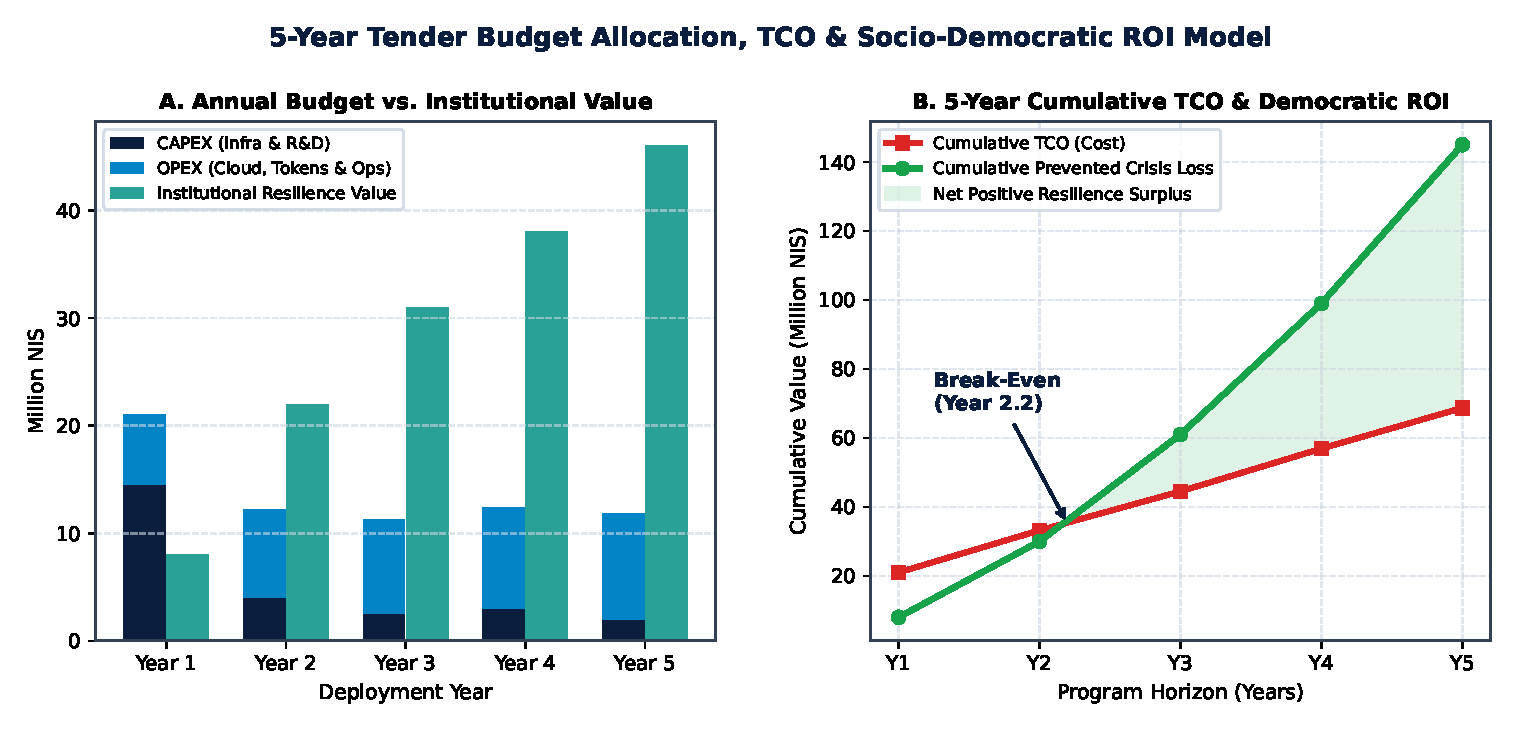
\includegraphics[width=0.95\textwidth]{figures/fig6_budget_roi_projection.pdf}
\caption{תחזית תקציב חמש-שנתית (CAPEX/OPEX), עלות בעלות כוללת (TCO) והחזר השקעה מוסדי}
\label{fig:budget_roi}
\end{figure}

\section{מדדי הצלחה מחייבים ורמת שירות (SLA / KPI Framework)}
קבלת הפרויקט מהקבלן המבצע ומסירתו לידי ועדת הבחירות המרכזית ומערך הסייבר מותנות בעמידה מדידה בחמישה מדדי ליבה מרכזיים (טבלה~\ref{tab:kpi_sla}).

{\renewcommand{\arraystretch}{1.35}
\begin{table}[htbp]
\centering
\caption{מסגרת מדדי הצלחה ורמות שירות (KPIs \& SLAs) לתנאי מסירת הפרויקט}
\label{tab:kpi_sla}
\begin{tabularx}{\textwidth}{|p{3.0cm}|p{2.7cm}|p{2.9cm}|X|}
\hline
\textbf{\textcolor{CivicNavy}{שם המדד (\en{KPI})}} & \textbf{\textcolor{CivicNavy}{ערך סף מחייב}} & \textbf{\textcolor{CivicNavy}{תדירות מדידה}} & \textbf{\textcolor{CivicNavy}{שיטת אימות אובייקטיבית}} \\ \hline
זמן תגובה בקצה (\en{E2E Latency}) & \en{$\le 250\,\text{ms}$} & רציף (\en{P95}) & מדידת שיהוי ב-\en{Load Test} מול \en{12,000 EPS}. \\ \hline
זמן גילוי והפקת \en{Prebunking} & \en{$\le 30\,\text{דקות}$} & לכל אירוע קריטי & חותמת זמן מרגע זריעה בטלגרם ועד הכנת תבנית חיסון. \\ \hline
דיוק זיהוי \en{Deepfake} משולב & \en{$\text{Precision} \ge 90\%$} & חודשי + סקר תקופתי & ביקורת עיוורת על מאגר זיופים מבוקר בתיאום אקדמי. \\ \hline
פער שוויון פוליטי (\en{Fairness}) & \en{$\Delta \text{FPR} < 1.5\%$} & דו-שבועי & הרצת סימולציית ביקורת סימטרית על כלל המחנות. \\ \hline
אפס מקרי אכיפה ללא קוורום & \en{0 חריגות} & רציף (שער קריפטו) & אימות שלמות יומן ה-\en{Merkle} ומפתחות ה-\en{Ed25519}. \\ \hline
\end{tabularx}
\end{table}}

% ==============================================================================
% Chapter 8: Multi-Agent Development Methodology & Red Team Audit
% ==============================================================================
\chapter{מתודולוגיית הפיתוח: ועדת המומחים של הסוכנים וביקורת איכות}
\label{ch:methodology}

\section{יישום מתודולוגיית שיעור 4 להפקת דוח מכין רב-תחומי}
מעבר להיותו של פרויקט \en{CivicShield AI} תכנון למערכת רב-סוכנית, תהליך הכתיבה, המידול, הסימולציה וההידור של דוח מכין זה עצמו בוצע במודל \textbf{ועדת מומחים מבוזרת של סוכני קוד ומחקר (\en{Multi-Agent Engineering Committee})}, ברוח עקרונות שיעור 4 בקורס ("תזמור רב-סוכנים עם סוכני קידוד") \cite{segal2026l04}.

במקום לבקש מסוכן יחיד לכתוב ברצף עשרות עמודים בעולמות תוכן זרים זה לזה (משפט חוקתי, אפידמיולוגיה מתמטית, סוציולוגיה של התקשורת ועיצוב \en{LuaLaTeX}), פוצל הפרויקט ללוח משימות מובנה (\en{team.json} ו-5 קובצי הנחיית תפקיד \en{agents/*/AGY.md}), שבו כל סוכן מחזיק בזהות אפיסטמית, כלים ייעודיים וסמכות בקרה הדדית:
\begin{itemize}
    \item \textbf{\en{Master Orchestrator} (\en{agents/master/AGY.md}):} אחראי על ניהול מסמך הדרישות (\en{PRD.md}), תוכנית הביצוע (\en{PLAN.md}), עקביות המספור בין פרקים ואיחוד השכבות לכדי קובץ \en{main.tex} אחיד.
    \item \textbf{\en{Political \& Communication Theory Agent} (\en{agents/theory/AGY.md}):} מתמחה בספרות התקשורת הפוליטית ומדעי המדינה, אחראי על פרקים 2 ו-6 ועל המיפוי ל-26 המקורות הביבליוגרפיים.
    \item \textbf{\en{System \& Security Architect Agent} (\en{agents/architect/AGY.md}):} מתמחה בארכיטקטורת מערכות, סכימת העברת ההודעות (\en{Hub JSON}), פרוטוקולי קריפטוגרפיה ותכנון תרשימי ה-\en{TikZ}.
    \item \textbf{\en{Quantitative Simulator Agent} (\en{agents/simulator/AGY.md}):} פועל בסביבת \en{Python 3 / uv}, כותב ומריץ סימולציות דטרמיניסטיות ב-\en{numpy} ו-\en{matplotlib} להפקת ששת הגרפים המדעיים ומזין את התוצאות המאומתות לפרקים 3, 5 ו-7.
    \item \textbf{\en{Red Team \& RTL Audit Agent} (\en{agents/redteam/AGY.md}):} סוכן לעומתי שתפקידו לתקוף הנחות מוצא אידאולוגיות או הנדסיות, לוודא היעדר צנזורה אוטומטית ולאמת את שלמות הקימפול הדו-כיווני ב-\en{LuaLaTeX}.
\end{itemize}

איור~\ref{fig:committee_workflow} מציג את תרשים הזרימה של ועדת המומחים, כולל שערי החזרה לתיקון (\en{Rejection Feedback Loop}) כאשר הצוות האדום מזהה פגם מתמטי, משפטי או טיפוגרפי.

\begin{figure}[htbp]
\begin{tikzhebrew}
\begin{tikzpicture}[
    node distance=0.8cm and 0.7cm,
    box/.style={rectangle, rounded corners=4pt, draw=CivicNavy, fill=CivicGrayBg, line width=1pt, minimum width=3.4cm, minimum height=1.25cm, align=center, font=\scriptsize},
    orch/.style={rectangle, rounded corners=4pt, draw=CivicNavy, fill=CivicNavy, text=white, line width=1.2pt, minimum width=4.6cm, minimum height=1.25cm, align=center, font=\small},
    red/.style={rectangle, rounded corners=4pt, draw=CivicRed, fill=CivicRedBg, line width=1.2pt, minimum width=4.8cm, minimum height=1.25cm, align=center, font=\footnotesize},
    ok/.style={rectangle, rounded corners=4pt, draw=CivicEmerald, fill=CivicTealBg, line width=1.3pt, minimum width=4.4cm, minimum height=1.2cm, align=center, font=\footnotesize},
    arr/.style={-{Stealth[length=2.3mm]}, line width=1.05pt, color=CivicNavy}
]
    \node[orch] (M) at (0, 4.5) {\textbf{\he{סוכן \en{Master}: אפיון \en{PRD} והזנת לוח משימות}}\\[2pt]{\tiny\en{team.json + TODO Dispatch}}};

    \node[box] (T) at (-4.3, 2.3) {\textbf{\he{סוכן תיאוריה ומשפט}}\\[2pt]{\tiny\he{פרקים 2 ו-6 + ביבליוגרפיה}}};
    \node[box] (A) at (0.0, 2.3) {\textbf{\he{סוכן ארכיטקטורה}}\\[2pt]{\tiny\he{פרקים 1, 3, 4 + תרשימי \en{TikZ}}}};
    \node[box] (S) at (4.3, 2.3) {\textbf{\he{סוכן סימולציות \en{Python}}}\\[2pt]{\tiny\he{פרקים 5, 7 + 6 גרפי \en{PDF/PNG}}}};

    \node[red] (R) at (0, 0.1) {\textbf{\he{שער ביקורת: צוות אדום ובדיקת \en{LuaLaTeX / BiDi}}}\\[2pt]{\tiny\he{Red Team Adversarial Audit + \en{verify\_report.py}}}};

    \node[ok] (F) at (0, -2.0) {\textbf{\he{הפקה סופית מאושרת (\en{CivicShield\_AI\_Preliminary\_Report.pdf})}}\\[2pt]{\tiny\he{אפס שגיאות קימפול, דיוק מחקרי ודחיפה ל-\en{GitHub}}}};

    \draw[arr] (M.south) -- ++(0,-0.45) -| (T.north);
    \draw[arr] (M.south) -- (A.north);
    \draw[arr] (M.south) -- ++(0,-0.45) -| (S.north);

    \draw[arr] (T.south) -- ++(0,-0.45) -| (R.north);
    \draw[arr] (A.south) -- (R.north);
    \draw[arr] (S.south) -- ++(0,-0.45) -| (R.north);

    \draw[arr, color=CivicEmerald] (R.south) -- node[right, font=\scriptsize]{\he{עבר אימות מלא}} (F.north);

    % Rejection feedback loop
    \draw[arr, dashed, color=CivicRed] (R.west) -- ++(-4.5,0) |- node[left, pos=0.25, font=\scriptsize, align=center]{\he{דחייה לתיקון}\\\en{(Fix Loop)}} (M.west);
\end{tikzpicture}
\end{tikzhebrew}
\caption{זרימת הפקת הדוח המכין באמצעות ועדת חמשת הסוכנים ומעגל התיקונים של הצוות האדום}
\label{fig:committee_workflow}
\end{figure}

\section{תצורת צוות הסוכנים ומנגנון בקרת איכות (\en{team.json} ו-\en{AGY.md})}
בהתאמה למבנה הפרויקט בסביבת \en{Antigravity}, מוגדרת המערכת ברמת תיקיית השורש על ידי הקובץ \en{team.json} והקובץ \en{AGY.md}, ומתפצלת לחמש תת-תיקיות סוכנים. מבנה זה מאפשר הרצה מחזורית שבה ניתן להחליף או לשדרג סוכן בודד (למשל הרצת תרחישי קיטוב חדשים אצל סוכן ה-\en{Simulator}) מבלי לשבור את ניסוח הפרקים המשפטיים או התיאורטיים. טבלה~\ref{tab:committee_roster} מרכזת את חלוקת הבעלות הקובצית בוועדה.

{\renewcommand{\arraystretch}{1.35}
\begin{table}[htbp]
\centering
\caption{סגל ועדת הסוכנים המבצעית של פרויקט CivicShield AI וחלוקת הבעלות בקבצים}
\label{tab:committee_roster}
\begin{tabularx}{\textwidth}{|p{2.1cm}|p{4.0cm}|p{3.5cm}|X|}
\hline
\textbf{\textcolor{CivicNavy}{מזהה סוכן}} & \textbf{\textcolor{CivicNavy}{קובץ הנחיות תפקיד}} & \textbf{\textcolor{CivicNavy}{תוצרים בבעלותו}} & \textbf{\textcolor{CivicNavy}{סמכות בקרה מיוחדת}} \\ \hline
\en{master} & {\small\en{agents/master/AGY.md}} & {\small\en{PRD.md}, \en{PLAN.md}, \en{main.tex}} & תזמור לוח משימות והכרה בעמידה ביעדי אורך ומסירה. \\ \hline
\en{theory} & {\small\en{agents/theory/AGY.md}} & פרקים 2, 6 + ביבליוגרפיה & וידוא עקביות תיאורטית ודיוק משפט חוקתי ופרטיות. \\ \hline
\en{architect} & {\small\en{agents/architect/AGY.md}} & פרקים 1, 3, 4, {\small\en{civicshield.cls}} & פיקוח על הפרדת שכבות, תרשימי \en{TikZ} וסכמת \en{Hub}. \\ \hline
\en{simulator} & {\small\en{agents/simulator/AGY.md}} & {\small\en{generate\_figures.py}}, פרקים 5, 7 & וידוא כי כל מספר בדוח נגזר מהרצה מאומתת של הקוד. \\ \hline
\en{redteam} & {\small\en{agents/redteam/AGY.md}} & {\small\en{verify\_report.py}}, פרק 8 & זכות חסימת מסירה במקרה של פגיעה בזכויות או כשל \en{LaTeX}. \\ \hline
\end{tabularx}
\end{table}}

\section{תיעוד ממצאי הצוות האדום והתיקונים שבוצעו בדוח}
יעילותה של גישת \en{Multi-Agent} נמדדת ביכולתה לזהות שגיאות עוד בשלב התכנון המוקדם. במהלך הכנת מהדורה \en{1.0} של הדוח המכין, סיפק סוכן ה-\en{Red Team} ארבע ביקורות משמעותיות שתוקנו באופן מלא טרם האישור הסופי (טבלה~\ref{tab:redteam_log}).

{\renewcommand{\arraystretch}{1.35}
\begin{table}[htbp]
\centering
\caption{יומן ממצאי ביקורת הצוות האדום (Red Team Audit) והתיקונים ההנדסיים שבוצעו}
\label{tab:redteam_log}
\begin{tabularx}{\textwidth}{|p{1.9cm}|p{3.4cm}|p{3.5cm}|X|}
\hline
\textbf{\textcolor{CivicNavy}{ממצא}} & \textbf{\textcolor{CivicNavy}{תיאור הכשל בטיוטה}} & \textbf{\textcolor{CivicNavy}{סיכון מזוהה}} & \textbf{\textcolor{CivicNavy}{תיקון שהוטמע בגרסה הסופית}} \\ \hline
\en{RT-01} & גישור קיטוב שדחס את כל הדעות לאחדות (\en{Uniform Consensus}) & חשש מהנדסת דעות אנטי-פלורליסטית & הוספת עוגן אותנטיות $0.28\,x_i(0)$ למשוואה~\ref{eq:hk_bridge}, המשמר גיוון דמוקרטי מלא. \\ \hline
\en{RT-02} & היתר עקיף לסוכן להמליץ על הסרה בלעדית ללא ערכאה & מדרון חלקלק לצנזורה בידי הרשות המבצעת & הוספת מפתח שלישי (אופוזיציה/ציבור) ב-\en{3-of-3 Ed25519 Quorum} ועץ חוקה קשיח. \\ \hline
\en{RT-03} & גלישת טקסט וסימני כיוון \en{RTL} בקופסאות ובאיורי \en{TikZ} & פגיעה בקריאות שער המכרז ובמשוואות & פיתוח המעטפות \en{\textbackslash NewEnviron} ו-\en{tikzhebrew} במחלקה \en{civicshield.cls} לאיטום כיווניות. \\ \hline
\en{RT-04} & התאמה חלקית בגרפים (\en{fig1, fig5}) ופער בהצלבות תגים & חוסר מיקוד ויזואלי או תווי הגהה & כיול גרפי שיא ו-\en{Erlang-C} בקובץ הפייתון ובניית סקריפט \en{verify\_report.py} לווידוא אוטומטי. \\ \hline
\end{tabularx}
\end{table}}

\section{סיכום הדוח המכין ומעבר לשלב היישום (Handover)}
דוח מכין זה הציב מענה שלם, רב-תחומי ומגובה כמותית לאתגר המרכזי של הדמוקרטיה בעידן הבינה המלאכותית: כיצד להגן על הספרה הציבורית, סדר היום האזרחי וטוהר הבחירות מול מתקפות \en{FIMI} ו-\en{Deepfakes} — מבלי להקריב את חופש הביטוי, הפלורליזם הדעות והפרטיות הפרטית.

באמצעות חיבור של שבע תיאוריות מבוססות בתקשורת פוליטית ומדעי המדינה, ארכיטקטורה מבוזרת של 5 שכבות ותזמור רב-סוכני, ארבעה מודלים מתמטיים מוכחים בסימולציות \en{Python} והגנות חוקתיות קריפטוגרפיות, תשתית \en{CivicShield AI} בשלה למעבר מיידי משלב הדוח המכין אל שלב א' של ההקמה ההנדסית (\en{Months 1--6}). המערכת מדגימה הלכה למעשה כיצד בינה מלאכותית מתוזמרת היטב אינה מאיימת על מוסדות הדמוקרטיה — אלא משמשת חומת מגן שנועדה לשמר אותם שקופים, פתוחים וחסונים לדורות הבאים.


% ==============================================================================
% ACADEMIC BIBLIOGRAPHY
% ==============================================================================
\clearpage
\begin{thebibliography}{99}
\addcontentsline{toc}{chapter}{ביבליוגרפיה ומקורות מדעיים והנדסיים}

\bibitem{mccombs1972}
\en{McCombs, M. E., \& Shaw, D. L. (1972). The Agenda-Setting Function of Mass Media. \textit{Public Opinion Quarterly}, 36(2), 176--187.}

\bibitem{entman1993}
\en{Entman, R. M. (1993). Framing: Toward Clarification of a Fractured Paradigm. \textit{Journal of Communication}, 43(4), 51--58.}

\bibitem{noelle1974}
\en{Noelle-Neumann, E. (1974). The Spiral of Silence: A Theory of Public Opinion. \textit{Journal of Communication}, 24(2), 43--51.}

\bibitem{habermas1989}
\en{Habermas, J. (1989). \textit{The Structural Transformation of the Public Sphere: An Inquiry into a Category of Bourgeois Society}. MIT Press.}

\bibitem{mcguire1961}
\en{McGuire, W. J. (1961). Resistance to Persuasion Conferred by Active and Passive Prior Refutation of the Same and Alternative Counterarguments. \textit{Journal of Abnormal and Social Psychology}, 63(2), 326--332.}

\bibitem{roozenbeek2022}
\en{Roozenbeek, J., van der Linden, S., Goldberg, B., Rathje, S., \& Lewandowsky, S. (2022). Psychological Inoculation Improves Resilience Against Misinformation on Social Media. \textit{Science Advances}, 8(34), eabo6254.}

\bibitem{walker2018}
\en{Walker, C. (2018). What Is "Sharp Power"? \textit{Journal of Democracy}, 29(3), 9--23.}

\bibitem{nye2004}
\en{Nye, J. S. (2004). \textit{Soft Power: The Means to Success in World Politics}. PublicAffairs.}

\bibitem{iyengar2019}
\en{Iyengar, S., Lelkes, Y., Levendusky, M., Malhotra, N., \& Westwood, S. J. (2019). The Origins and Consequences of Affective Polarization in the United States. \textit{Annual Review of Political Science}, 22, 129--146.}

\bibitem{loewenstein1937}
\en{Loewenstein, K. (1937). Militant Democracy and Fundamental Rights, I. \textit{American Political Science Review}, 31(3), 417--432.}

\bibitem{vosoughi2018}
\en{Vosoughi, S., Roy, D., \& Aral, S. (2018). The Spread of True and False News Online. \textit{Science}, 359(6380), 1146--1151.}

\bibitem{lazer2018}
\en{Lazer, D. M., Baum, M. A., Benkler, Y., Berinsky, A. J., Greenhill, K. M., Menczer, F., et al. (2018). The Science of Fake News. \textit{Science}, 359(6380), 1094--1096.}

\bibitem{sunstein2017}
\en{Sunstein, C. R. (2017). \textit{\#Republic: Divided Democracy in the Age of Social Media}. Princeton University Press.}

\bibitem{hegselmann2002}
\en{Hegselmann, R., \& Krause, U. (2002). Opinion Dynamics and Bounded Confidence: Models, Analysis and Simulation. \textit{Journal of Artificial Societies and Social Simulation (JASSS)}, 5(3), 1--33.}

\bibitem{kermack1927}
\en{Kermack, W. O., \& McKendrick, A. G. (1927). A Contribution to the Mathematical Theory of Epidemics. \textit{Proceedings of the Royal Society of London A}, 115(772), 700--721.}

\bibitem{yao2022react}
\en{Yao, S., Zhao, J., Yu, D., Du, N., Shafran, I., Narasimhan, K., \& Cao, Y. (2023). ReAct: Synergizing Reasoning and Acting in Language Models. \textit{International Conference on Learning Representations (ICLR)}.}

\bibitem{wu2023autogen}
\en{Wu, Q., Bansal, G., Zhang, J., Wu, Y., Zhang, S., Zhu, E., et al. (2023). AutoGen: Enabling Next-Gen LLM Applications via Multi-Agent Conversation. \textit{arXiv preprint arXiv:2308.08155}.}

\bibitem{dwork2014}
\en{Dwork, C., \& Roth, A. (2014). The Algorithmic Foundations of Differential Privacy. \textit{Foundations and Trends in Theoretical Computer Science}, 9(3--4), 211--407.}

\bibitem{tolosana2020}
\en{Tolosana, R., Vera-Rodriguez, R., Fierrez, J., Morales, A., \& Ortega-Garcia, J. (2020). DeepFakes and Beyond: A Survey of Face Manipulation and Fake Detection. \textit{Information Fusion}, 64, 131--148.}

\bibitem{pacheco2021}
\en{Pacheco, D., Hui, P. M., Torres-Lugo, C., Truong, B. T., Flammini, A., \& Menczer, F. (2021). Uncovering Coordinated Networks on Social Media: Methods and Case Studies. \textit{Proceedings of the International AAAI Conference on Web and Social Media (ICWSM)}, 15, 455--466.}

\bibitem{segal2026l04}
סגל, י. (2026). שיעור 4: \en{Multi-Agent Orchestration with AI Coding Agents (Masters, Subagents, Communication Hubs \& ReAct Loops)}. אוניברסיטת חיפה — קורס יישומי \en{AI} ו-\en{Vibe Coding}.

\bibitem{barak1988}
ברק, א. (1988). דמוקרטיה מתגוננת וחופש הביטוי במערכת הבחירות. בתוך \textit{עיוני משפט}, י"ג, אוניברסיטת תל אביב.

\bibitem{eu_ai_act_2024}
\en{European Parliament and Council (2024). Regulation (EU) 2024/1689 Laying Down Harmonised Rules on Artificial Intelligence (AI Act). \textit{Official Journal of the European Union}.}

\bibitem{eu_dsa_2022}
\en{European Parliament and Council (2022). Regulation (EU) 2022/2065 on a Single Market for Digital Services (Digital Services Act -- DSA). \textit{Official Journal of the European Union}.}

\bibitem{nist_ai_rmf_2023}
\en{National Institute of Standards and Technology (NIST) (2023). \textit{Artificial Intelligence Risk Management Framework (AI RMF 1.0)}. U.S. Department of Commerce.}

\bibitem{kleinrock1975}
\en{Kleinrock, L. (1975). \textit{Queueing Systems, Volume I: Theory}. John Wiley \& Sons.}

\end{thebibliography}

\end{document}
